\documentclass[12pt]{article}
\usepackage{graphicx} 
\usepackage[utf8]{inputenc}
\usepackage[a4paper,bindingoffset=0.2in,left=1.3in,right=1.3in,top=1.3in,bottom=1.3in]{geometry}
\usepackage{hyperref}
\usepackage{dirtytalk}
\usepackage{biblatex}
\addbibresource{bibliography.bib}
\usepackage{verbatim}
\usepackage{wrapfig}
\usepackage{multirow}

\usepackage{url}
\setcounter{biburllcpenalty}{7000}
\setcounter{biburlucpenalty}{8000}

\usepackage{titlesec}
\titleclass{\subsubsubsection}{straight}[\subsection]

\newcounter{subsubsubsection}[subsubsection]
\renewcommand\thesubsubsubsection{\thesubsubsection.\arabic{subsubsubsection}}
\renewcommand\theparagraph{\thesubsubsubsection.\arabic{paragraph}} % optional; useful if paragraphs are to be numbered

\titleformat{\subsubsubsection}
  {\normalfont\normalsize\bfseries}{\thesubsubsubsection}{1em}{}
\titlespacing*{\subsubsubsection}
{0pt}{3.25ex plus 1ex minus .2ex}{1.5ex plus .2ex}

\makeatletter
\renewcommand\paragraph{\@startsection{paragraph}{5}{\z@}%
  {3.25ex \@plus1ex \@minus.2ex}%
  {-1em}%
  {\normalfont\normalsize\bfseries}}
\renewcommand\subparagraph{\@startsection{subparagraph}{6}{\parindent}%
  {3.25ex \@plus1ex \@minus .2ex}%
  {-1em}%
  {\normalfont\normalsize\bfseries}}
\def\toclevel@subsubsubsection{4}
\def\toclevel@paragraph{5}
\def\toclevel@paragraph{6}
\def\l@subsubsubsection{\@dottedtocline{4}{7em}{4em}}
\def\l@paragraph{\@dottedtocline{5}{10em}{5em}}
\def\l@subparagraph{\@dottedtocline{6}{14em}{6em}}
\makeatother

\setcounter{secnumdepth}{4}
\setcounter{tocdepth}{4}

\makeatletter
\let \@sverbatim \@verbatim
\def \@verbatim {\@sverbatim \verbatimplus}
{\catcode`'=13 \gdef \verbatimplus{\catcode`'=13 \chardef '=13 }} 
\makeatother


\begin{document}

\begin{titlepage}

\begin{center}

\hspace{0pt}\\

\vspace{1.5cm}
{{\huge\textbf{Analysis of MySQL DBMS with InnoDB Engine}}}\\
\vspace{0.5cm}
{\Large Database Systems}\\[5pt]
{\Large FCT NOVA}\\[4pt]
\vspace{1.5cm}

\begin{figure}[h]
    \centering
    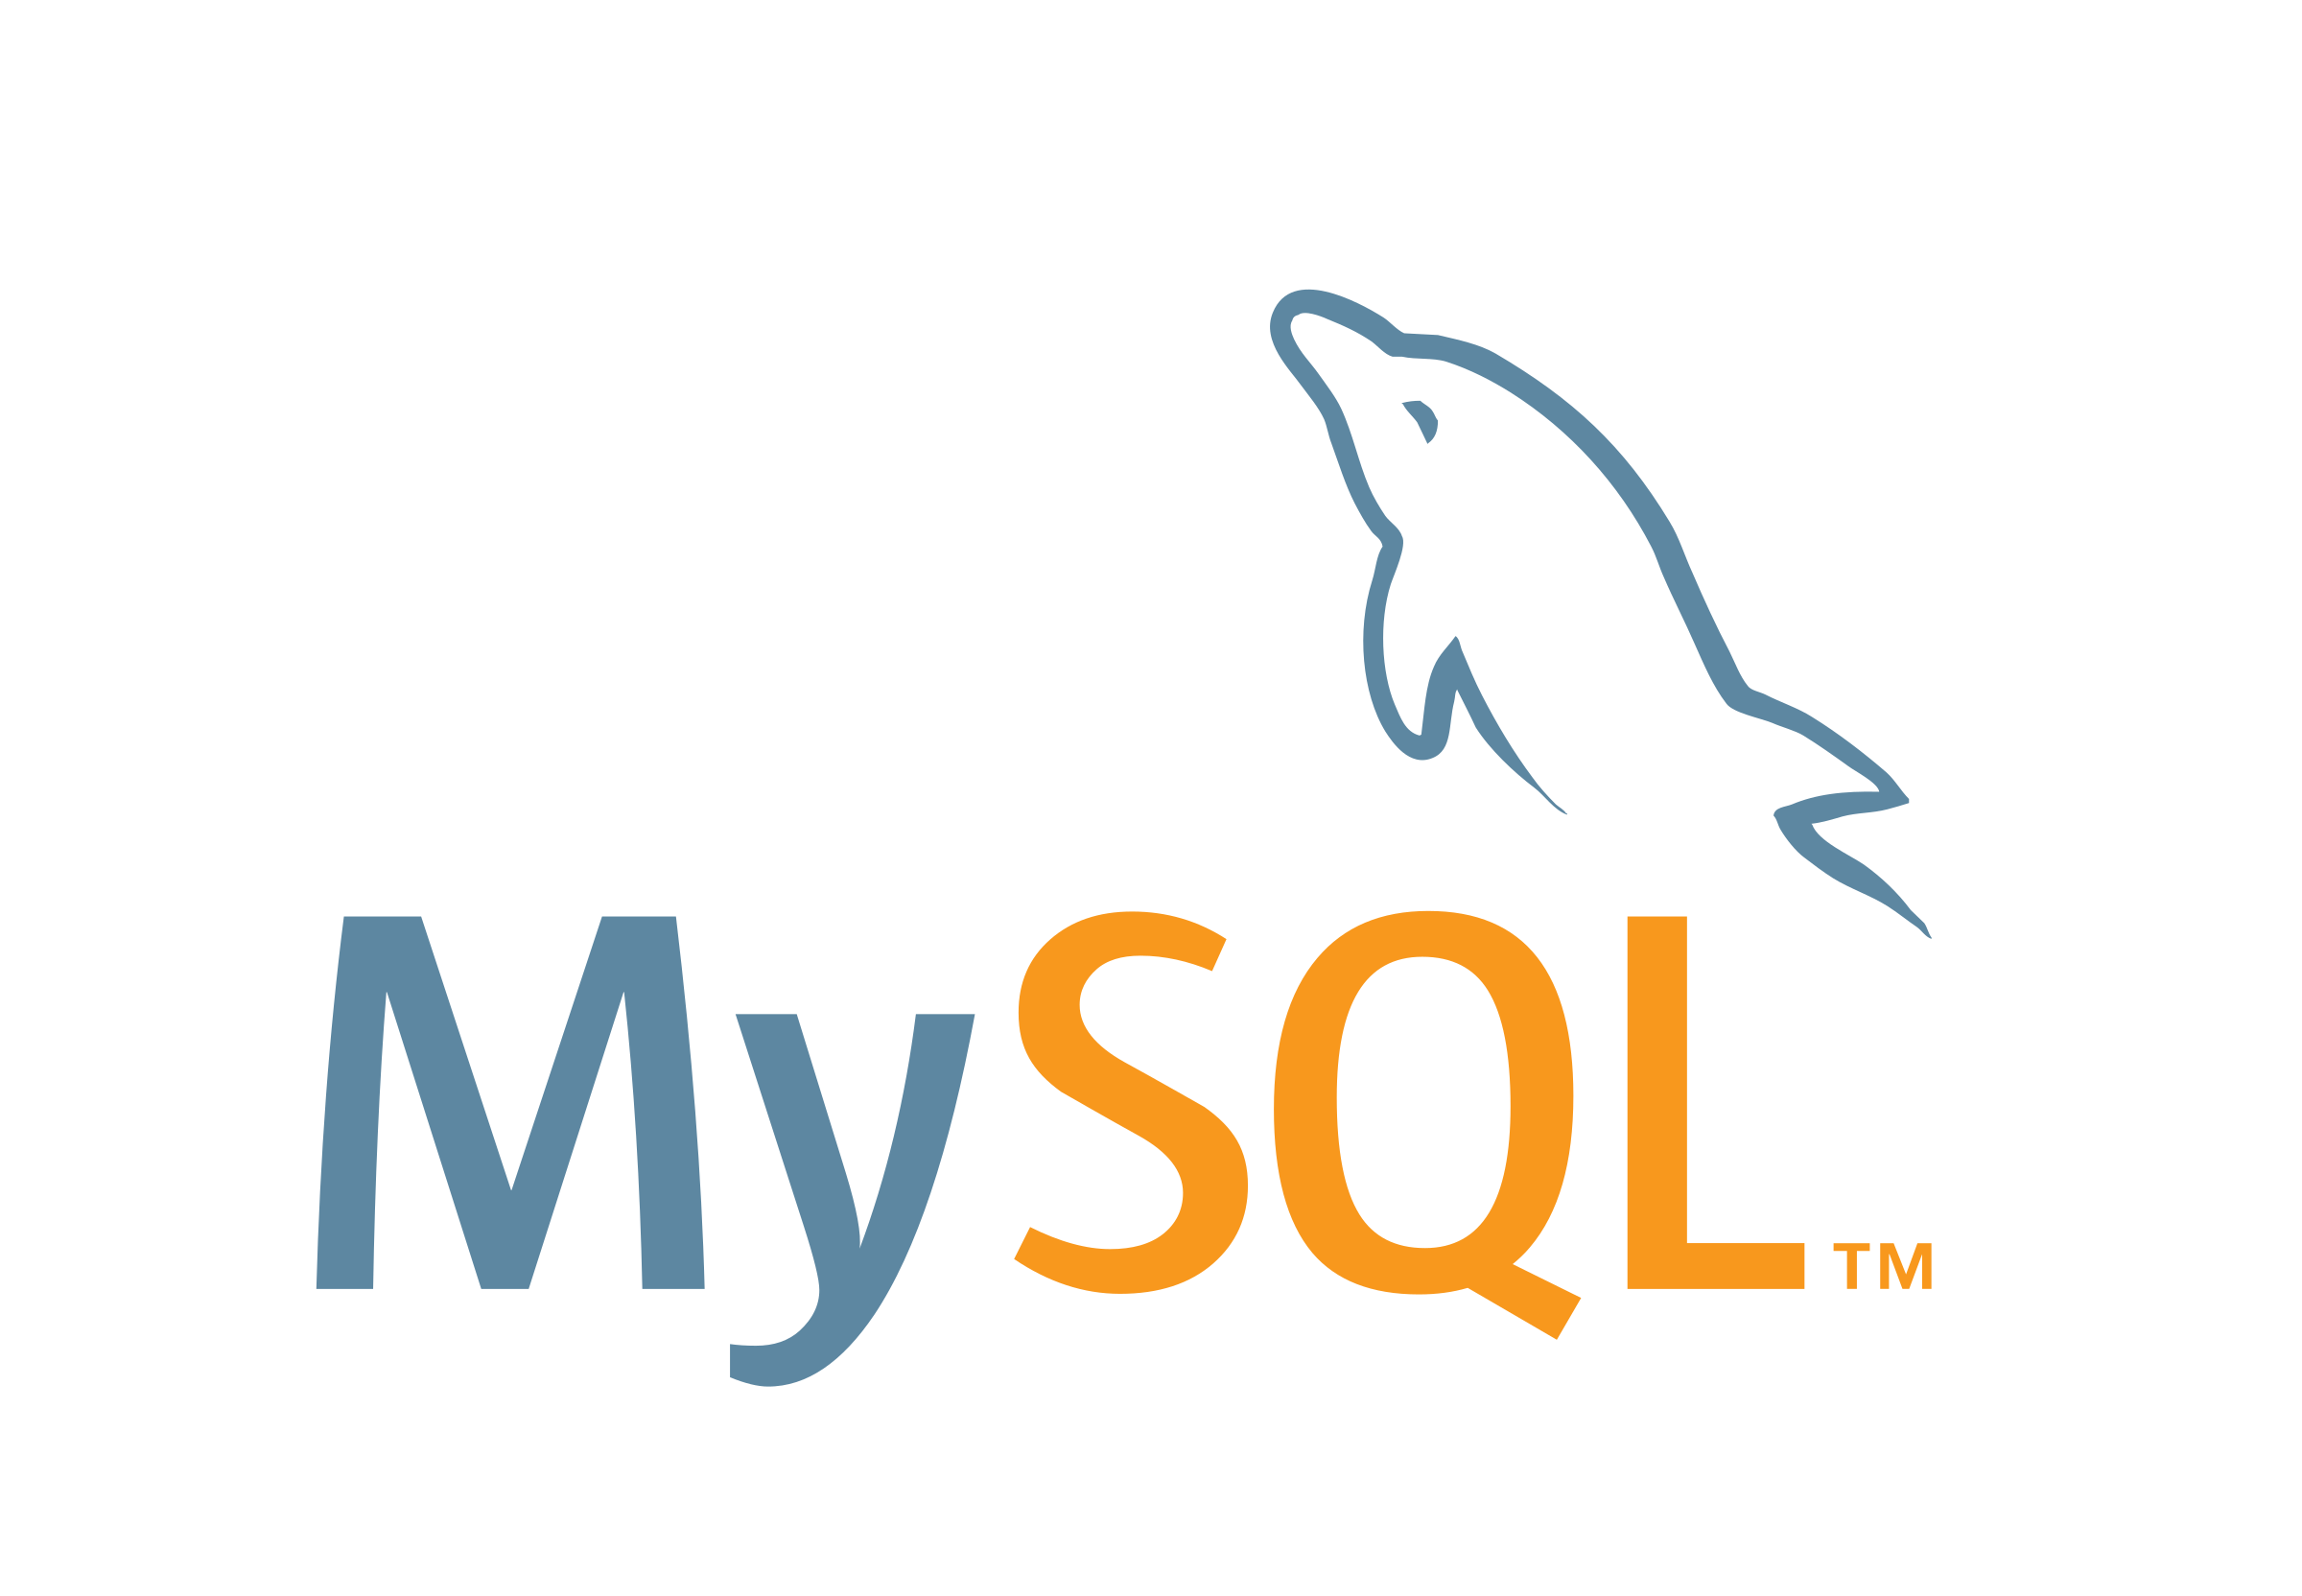
\includegraphics[scale=.17]{files/mysql-logo.png}
\end{figure}

\vspace{5cm}
%{Ema Vieira, number 50095}\\
%{Giovanna Lopez, number 50265}\\
%{André Atalaia, number 51910}\\

\vspace{2cm}
{{22nd of may, 2020}}\\

\end{center}
\end{titlepage}

\newpage
\tableofcontents


\newpage
\section{Introduction}
\label{intro}
For this project, we chose to study MySQL 8.0 based on its popularity and due to the fact that we are using it as our main database in other Computer Science courses.

As we will explain in detail in Section \ref{storageEngines}, MySQL supports several storage engines. However, for the purpose of this project, we will focus our analysis on the InnoDB storage engine, as it currently is the default for MySQL.


\subsection{Report Structure}
\label{structure}
What follows is a very short summary of the contents discussed in each section of this report:

\vspace{0.3cm}

In Section \ref{storage}, we talk about the storage and file structure used in MySQL. We start by specifying the various storage engines, and then go into detail only with InnoDB. We discuss MySQL's file system, tuple organization, buffer management and partitioning.

\vspace{0.2cm}

In Section \ref{indexingHashing}, we discuss how MySQL implements indexing and hashing. We talk about the index structures it implements and focus our explanation mainly on clustered and secondary indexes.

\vspace{0.2cm}

In Section \ref{queryProcessingOptimization}, we talk about the whole pipeline of how MySQL processes, optimizes and executes SQL queries. We focus mainly on the optimization aspect, by describing the several ways in which the query optimizer can optimize queries, namely optimizing through indexes and optimizing simple and complex operations. We also explain how the Query optimizer can be controlled, how MySQL estimates table and index statistics and how the user can see information about the execution plan.

\vspace{0.2cm}

In Section \ref{transactionAndConcurrency}, we talk about MySQL transactions and how they adhere to the ACID model, explaining how each property is implemented in detail. We also describe how MySQL controls concurrency by the using locks.

\vspace{0.2cm}

Seen as the InnoDB storage engine does not offer support for distributed databases, that subject is not covered in this report.

\vspace{0.2cm}

Additionally, in Section \ref{otherCharacteristics}, we describe some interesting characteristics of MySQL. We talk about MySQL's support for XML and XPath, and its implementation of stored routines and triggers. We also discuss how to use JDBC to connect to a MySQL database, and present a very useful graphical tool, MySQL Workbench.

\vspace{0.2cm}

Please note that all sections, except Section \ref{otherCharacteristics}, end with a comparison of MySQL to Oracle regarding the subjects studied in that section.

\newpage 

\subsection{History of MySQL}
\label{history}
MySQL is the world's most popular open source Database Management System (DBMS) and it is currently developed, distributed and supported by Oracle Corporation \parencite{WHATIS}. It has great performance, reliability, ease-of-use and has become the leading database choice for web-based applications. It is used by high profile companies such as Facebook, Twitter and YouTube.

\vspace{0.3cm}

MySQL was born in Sweden, in the 90's, at a company founded by David Axmark, Allan Larsson and Michael Widenius. The creators felt the need to connect their tables to a database, mSQL, using Indexed Sequential Access Method (ISAM) routines. However, mSQL was not fast nor flexible enough for their needs, so they created a new SQL interface.

MySQL was an open source project from the beginning but, when its popularity and number of users increased within the database community, it was bought by Sun Microsystems (2008). Later, this company was acquired by Oracle Corporation (2009). 

Nowadays, MySQL still belongs to Oracle Corporation and it comes in several editions \parencite{EDITIONS}. Some of these editions are free of charge and open source, and others are paid and come with additional functionalities.





\newpage
\section{Storage and File Structure}
\label{storage}
As we mentioned in Section \ref{intro}, this project will focus on the InnoDB storage engine. However, in Section \ref{storageEngines}, we will give some details about the various storage engines supported. 
Then, we will discuss MySQL's file system, tuple organization and, finally, we will detail how MySQL manages caching by using the buffer pool, and the various ways of partitioning it allows.

\subsection{Storage Engines}
\label{storageEngines}
MySQL is known for supporting multiple storage engines \parencite{ENGINES}. These storage engines are software components that a DBMS uses to handle SQL operations like create, read, update and delete (CRUD) for different table types. In other words, the DBMS uses storage engines as a way to manage the data in the underlying memory and storage systems \parencite{GUIDE_ENGINES}, providing an abstraction layer that prevents contact between the users and the native file system.

\vspace{0.3cm}

\noindent Below, we present the storage engines supported by MySQL 8.0:
\begin{itemize}
    \item \textbf{InnoDB:} This engine is the default in MySQL 5.5 and later. It is ACID compliant, having commit, rollback and crash-recovery capabilities. It supports row-level locking and multi-version concurrency control and it is the only engine that provides foreign key referential-integrity constraints;
    
    \item \textbf{MyISAM:} This engine uses table-level locking and, as such, it has very limited performance when it comes to read/write workloads, so it is mostly used in read-only or read-mostly workloads;
    
    \item \textbf{Memory:} This engine, formerly known as HEAP engine, stores all data in RAM to improve access speeds. As of late, it is not being used frequently because other engines have evolved in ways that match the access speed requirements; 
    
    \item \textbf{CSV:} This engine has tables (text files with comma-separated values) that let you import or dump data in CSV format;
    
    \item \textbf{Archive:} This engine has compact unindexed tables used for storing and retrieving large amounts of rarely used information;
    
    \item \textbf{Blackhole:} This engine accepts but does not store data so, queries always return an empty set. It is often used in distributed environments for replicating data with the master-slave model;

    \item \textbf{NDB aka NDBCLUSTER:} This clustered database engine is mostly used in distributed environments that have high uptime and availability needs;
    
    \item \textbf{Merge:} This engines allows the grouping of identical MyISAM tables;
    
    \item \textbf{Federated:} This engine is commonly used in distributed environments, because it allows the creation of a logical database by linking several physical MySQL servers;
    
    \item \textbf{Example:} This engine, present in the source code for MySQL, is an example that shows how to begin writing new storage engines.
    
\end{itemize}

The choice of storage engine greatly impacts the performance of the application, so choosing the right one is very important. The users should take into account the requirements of the application and the characteristics of each storage engine, in order to choose the one that better suits their needs. The code below shows how to set the default storage engine for a session \parencite{SET_ENGINE}:
\begin{verbatim}
    SET default_storage_engine = INNODB;
\end{verbatim}

It is important to note that the user is not restricted to using the same storage engine for an entire server or schema. The users can specify the storage engine for any table like so:
\begin{verbatim}
    CREATE TABLE t1 (i INT) ENGINE = CSV;
\end{verbatim}

When the \verb|ENGINE| option is omitted, the default storage engine is used. If the user did not set the default engine, InnoDB will be used. It is also possible to convert a table from one storage engine to another:
\begin{verbatim}
    ALTER TABLE t1 ENGINE = INNODB;
\end{verbatim}



\subsection{File System}
\label{filesystem}
InnoDB implements a storage system that has physical and logical characteristics to enhance performance, scalability and backup.

The System tablespace is the storage area for the change buffer. This buffer caches changes to secondary index pages when those pages are not in the buffer pool \parencite{ChangeBuffer}. 

By default, InnoDB stores both table and index data in a File-Per-Table tablespace, by creating a .ibd file per table \parencite{FileperTable}. If the user does not wish to store table and index data in a File-Per-Table tablespace, InnoDB allows him to choose other methods of storage, such as \parencite{CreatingTablesInnoDB}:
\begin{itemize}
    \item  \textbf{Storage in the System tablespace:} Keeping all InnoDB table and index data in one file, often causing it to become very large. The System tablespace never shrinks and, because of this, storage problems can arise if large amounts of temporary data are loaded and then deleted;
    \item \textbf{Storage in a General tablespace:} Keeping all InnoDB table and index data in a shared tablespace that supports all row formats and can be created like so:
    
\begin{verbatim}
CREATE TABLESPACE ts ADD DATAFILE 'ts.ibd' ENGINE = INNODB;
\end{verbatim}
    
\end{itemize}

As can be seen in Figure \ref{tablespaceImage}, each InnoDB tablespace stores rows inside pages. These pages have a default size of 16KB, but you can reduce it down to 4 or 8KB, or increase it to 32 or 64KB. 
The pages are then grouped into extents of size 1MB per 16KB in page size (e.g. If pages have 32KB, the extent size is 2MB) \parencite{FileSpaceManagement}.

\begin{figure}[h]
\centering
    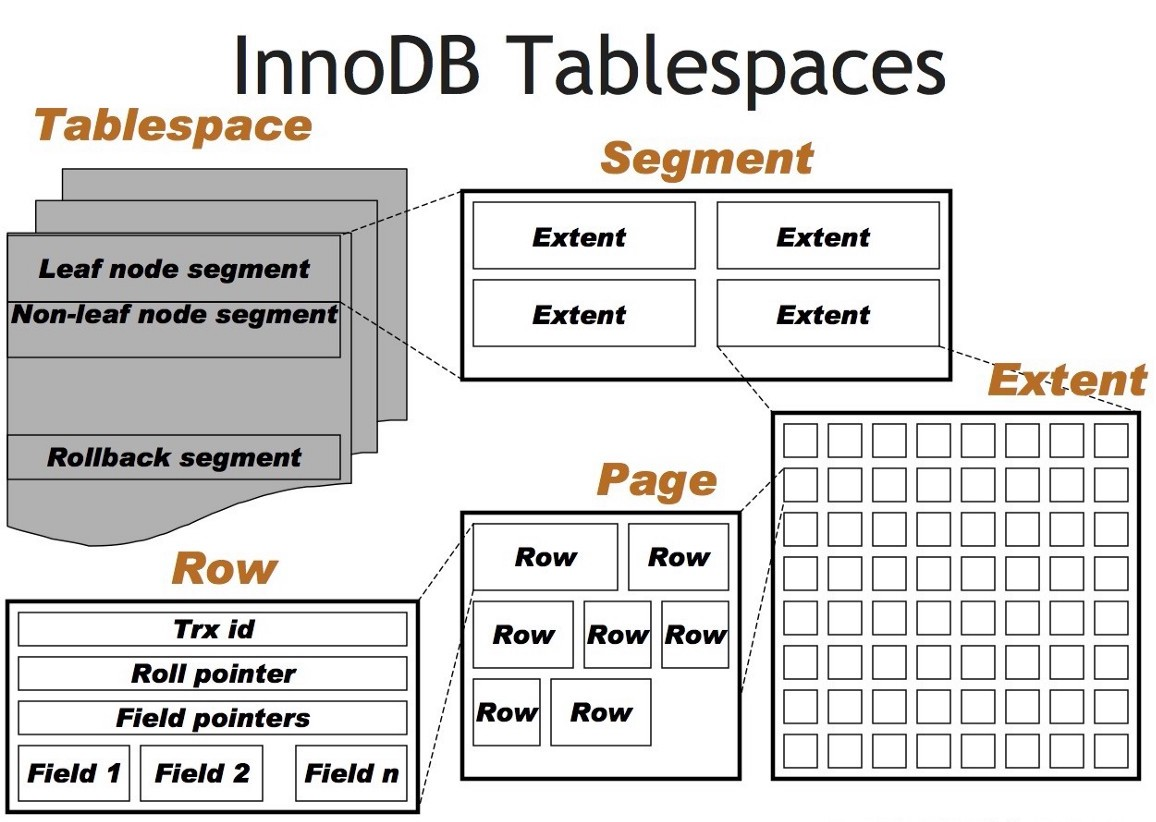
\includegraphics[scale=0.3]{files/tablespace.jpeg}
    \caption{Visual representation of InnoDB tablespaces. Adapted from \parencite{tablespaceImageLink}.}
    \label{tablespaceImage}
\end{figure}

In turn, the extents are grouped into \say{files} inside a tablespace called segments. When these segments grow, InnoDB allocates the first 32 pages to it one at a time. After that, it starts allocating whole extents to the segment. This can go up to a maximum of 4 extents at a time.

Each index is allocated two segments:
\begin{enumerate}
    \item A segment for non-leaf nodes of the B+-tree;
    \item A segment for the leaf nodes of the B+-tree.
\end{enumerate}



If the leaf nodes are kept in contiguous memory on disk, the sequential I/O operations will be better because they contain the actual table data.

When you delete data from a table, InnoDB shrinks the corresponding B+-tree indexes. The availability of the freed space depends on the pattern of deletes freeing individual pages or extents. On the other hand, when you delete all rows from a table or drop it, the space is guaranteed to be freed. 

It is important to note that, deleted rows are physically removed by the purge operation when they are no longer needed for transactions, rollbacks or consistent reads.



\subsection{Buffer Management}
\label{buffer}
The InnoDB engine reserves space in main memory for the buffer pool, a memory area where table and index data is cached when it is accessed. The buffer pool significantly speeds up the processing of data that is frequently used, so knowing how to manage it is extremely relevant for MySQL Database Tuning \parencite{BUFFER_POOL}.

The buffer pool is implemented as a linked-list of pages and, in order to manage the cache efficiently, a variation of the Least Recently Used (LRU) algorithm is used. As such, pages that are not frequently used tend to be removed from the buffer pool.

\subsubsection{Buffer Pool LRU Algorithm}
\label{LRU}
As we mentioned before, the buffer pool is managed by a variation of the LRU algorithm. When the buffer is full and someone accesses a page that is not in memory, that page needs to be inserted. 

The defining aspect of this variation is the midpoint insertion strategy - when inserting a new page, it is inserted in the middle of the list. This strategy divides the buffer pool in two sublists:

\begin{enumerate}
    \item At the head of the buffer pool is a sublist of new pages that were accessed recently;
    \item At the tail of the buffer pool is a sublist of old pages that were accessed less recently. These pages are the candidates for eviction.
\end{enumerate}

\begin{figure}[htbp]
\centering
    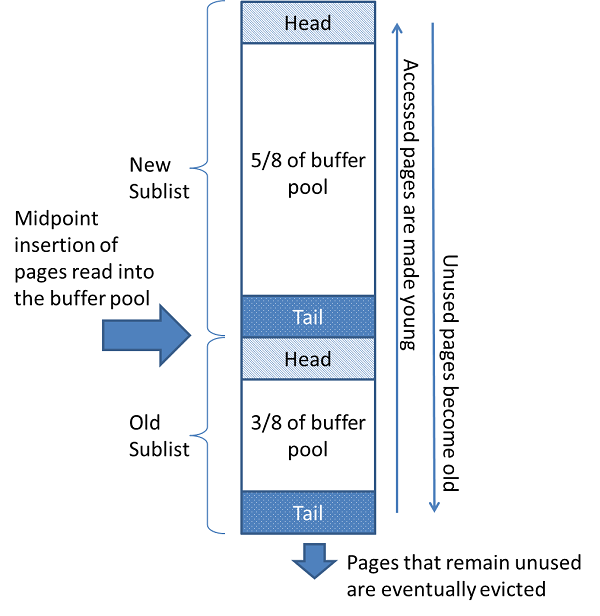
\includegraphics[scale=0.4]{files/buffer_pool.png}
    \caption{Visual representation of the Buffer Pool List and its division. Taken from MySQL Documentation page \parencite{BUFFER_POOL}.}
    \label{buffer_pool}
\end{figure}

The LRU algorithm reserves 3/8 of the buffer pool for the old sublist. When a page is read into the buffer, it is inserted at the midpoint. As can be seen in Figure \ref{buffer_pool}, this midpoint is not in the middle of the list. It is located on the boundary between the new page sublist and the old page sublist. When a page in the old sublist is accessed, it is moved to the head of the new sublist. 

As time passes, the pages that are not accessed keep moving toward the tail of the list. Pages in the new sublist \say{age} when other pages are made new. Pages in the old sublist \say{age} when other pages are made new and when pages are inserted at the midpoint. If a page is not used for a certain period of time, it tends to reach the tail of the old sublist, being evicted when a new page is inserted.

It is important to note that a page can be read because of a user-initiated operation or due to a read-ahead operation.

\subsubsection{Buffer Pool Configuration}
\label{bufferConfig}
The buffer pool can be configured in order to improve performance. There are several parameters that can be tuned, such as:
\begin{itemize}
    \item \textbf{Size of the buffer pool:} The size of the buffer pool should be set to as large a value as possible while still leaving enough memory for other processes. Obviously, if the buffer pool is very big, InnoBD reads data from disk only once and then is able to access it from memory. The size of the buffer pool can specified using the variable \verb|innodb_buffer_pool_size|;
    
    \item \textbf{Buffer pool instances:} If the \verb|innodb_buffer_pool_size| is set to a value larger than 1GB, it is possible to divide the buffer pool into various instances. This can significantly improve performance when concurrent threads are trying to read or write the cached pages. The number of buffer pool instances is set with \verb|innodb_buffer_pool_instances| and can vary between 1 and 64;
    
    \item \textbf{Resistance to scan:} When a table scan is performed, a large amount of data is brought into the buffer pool and a lot of older data is evicted, even if the new data is never used again. This can cause serious issues, so you can keep frequently accessed data in memory regardless of sudden spikes of activity. By setting \verb|innodb_old_blocks_time|, the time window (in milliseconds) after the first access to a page during which it can be accessed without being moved to the front of the LRU list, to a high value, our buffer will become table scan resistant;
    
    \item \textbf{Buffer pool prefetching:} Read-ahead requests prefetch pages into the buffer pool in anticipation that the pages will be needed soon. The \verb|innodb_read_ahead_threshold| and \verb|innodb_random_read_ahead| variables can control, respectively, when linear read-aheads and random read-aheads are performed;
    
    \item \textbf{Buffer pool flushing:} InnoDB performs the flushing of dirty pages from the buffer pool in the background. There are several parameters that can be controlled, such as the number of cleaner threads, \verb|innodb_page_cleaners|, and the low water mark for the percentage of dirty pages, \verb|innodb_max_dirty_pages_pct_lwm|;
    
    \item \textbf{Buffer pool state:} To avoid a large warm up period after restarting the server, a percentage of the most recently used pages for each buffer pool is saved at shutdown and restored at startup. This percentage can be set with the \verb|innodb_buffer_pool_dump_pct| variable.
    
\end{itemize}



\subsection{Tuple Organization}
\label{tuple}
In MySQL, the table data is divided into several pages. These pages are organized in a tree data structure called a B+-tree. This structure is used for storing both table data and secondary indexes \parencite{RowFormats}.

The B+-tree that represents a table is called the clustered index and is organized by the corresponding primary key columns. The nodes of the tree structure contain the values of all columns in the row. If the B+-tree is a secondary index, its nodes only contain the values of index columns and primary key columns.

If columns are of variable-length, also known as off-page columns, and are too long to fit on a B+-tree page, they are stored on separately allocated disk pages called overflow pages. Each column has a singly-linked list of one or more overflow pages. However, depending on column length, some column values may be stored in the B+-tree to avoid wasting storage and having to read a separate page.
MySQL variable length types are \verb|VARCHAR|, \verb|VARBINARY|, \verb|BLOB| and \verb|TEXT|.

\vspace{0.3cm}
InnoDB supports four row formats and we will talk about them in the following sections.

\subsubsection{REDUNDANT Row Format}
\begin{itemize}
    \item Provides compatibility with older versions of MySQL;
    \item Tables store the first 768 bytes of variable-length column values in the index record within the B+-tree node. The rest is stored on overflow pages;
    \item Fixed-length columns greater than or equal to 768 bytes are encoded as variable-length columns and are also stored off-page;
    \item For columns with values of 768 bytes or less, an overflow page is not used.
\end{itemize}


\subsubsection{COMPACT Row Format}
\begin{itemize}
    \item Reduces row storage space by about 20\% when compared to the REDUNDANT row format. However, it increases CPU usage for some operations;
    \item Tables store variable-length and fixed-length column values in the same way as the REDUNDANT row format.
\end{itemize}


\subsubsection{DYNAMIC Row Format}
\begin{itemize}
    \item Offers the same benefits as the COMPACT row format but enhances storage for long variable-length columns and supports large index key prefixes;
    \item Stores long variable-length column values completely off-page. The clustered index record contains only a 20-byte pointer to the overflow page;
    \item Fixed-length fields greater than or equal to 768 bytes are encoded as variable-length fields;
    \item The off-page storage depends on the page size and the total size of the row. The longest columns are chosen for off-page storage until the clustered index record fits on the B+-tree page;
    \item Tables can be stored in the System tablespace, File-per-Table tablespaces and General tablespaces.
\end{itemize}


\subsubsection{COMPRESSED Row Format}
\begin{itemize}
    \item Offers the same benefits as the DYNAMIC row format but supports table and index data compression;
    \item The \verb|KEY_BLOCK_SIZE| variable controls how much column data is stored in the clustered index, and how much is placed off-page;
    \item Tables can be stored in File-per-Table tablespaces and General tablespaces.
\end{itemize}



\subsection{Partitioning}
\label{partition}
Not all storage engines support the partitioning of tables. However, InnoDB is one of the engines that does \parencite{PARTITIONING}.

Partitioning allows the users to distribute the tables in portions across a file system, storing them as separate tables in different locations. This is done according to a rule chosen by the user, the partitioning function. This function relies on the partitioning type, which is also specified by the user.

Before delving into the partitioning types, it is important to note that:
\begin{itemize}
    \item The user cannot disable partitioning support in InnoDB;
    \item The same storage engine must be used for all partitions of the same partitioned table \parencite{PARTITIONING_OVERVIEW};
    \item The user must partition both table and indexes. It is also not possible to partition only a portion of a table.
\end{itemize}

There are two kinds of partitioning: the \textbf{horizontal partitioning}, where different rows of a table are assigned to different physical partitions, and \textbf{vertical partitioning}, where different columns of a table are assigned to different physical partitions. With this said, note that MySQL 8.0 does not support vertical partitioning.

Let us now look at the different horizontal partitioning types available in MySQL 8.0 \parencite{PARTITIONING_TYPES}.

\subsubsection{RANGE Partitioning}
When a table is partitioned by \verb|RANGE|, each partition contains rows for which the partitioning expression value lies within a given range. This is defined using the \verb|VALUES LESS THAN| operator.
To avoid getting an error when adding a row whose \verb|store_id| value is greater than the highest value defined, we use the \verb|MAXVALUE| operator \parencite{PARTITIONING_RANGE}:

\begin{verbatim}
CREATE TABLE employees (
    id INT NOT NULL,
    fname VARCHAR(30),
    lname VARCHAR(30),
    hired DATE NOT NULL DEFAULT '1970-01-01',
    separated DATE NOT NULL DEFAULT '9999-12-31',
    job_code INT,
    store_id INT
)
PARTITION BY RANGE (store_id) (
    PARTITION p0 VALUES LESS THAN (6),
    PARTITION p1 VALUES LESS THAN (11),
    PARTITION p2 VALUES LESS THAN (16),
    PARTITION p3 VALUES LESS THAN MAXVALUE
);\end{verbatim}

\subsubsection{LIST Partitioning}
This type of partitioning is similar to partitioning by \verb|RANGE| in the way that each partition must be explicitly defined. The big difference lies in the fact that, in \verb|LIST| partitioning, each partition is defined and selected based on if a column value belongs to a list of values and not to a contiguous range of values. 
To specify the list that will define each partition we use the \verb|VALUES IN| operator \parencite{PARTITIONING_LIST}:

\begin{verbatim}
CREATE TABLE employees (
    id INT NOT NULL,
    fname VARCHAR(30),
    lname VARCHAR(30),
    hired DATE NOT NULL DEFAULT '1970-01-01',
    separated DATE NOT NULL DEFAULT '9999-12-31',
    job_code INT,
    store_id INT
)
PARTITION BY LIST(store_id) (
    PARTITION pNorth VALUES IN (3,5,6,9,17),
    PARTITION pEast VALUES IN (1,2,10,11,19,20),
    PARTITION pWest VALUES IN (4,12,13,14,18),
    PARTITION pCentral VALUES IN (7,8,15,16)
);
\end{verbatim}

\subsubsection{COLUMNS Partitioning}
This partitioning is a variant on \verb|RANGE| and \verb|LIST| partitioning. \verb|COLUMNS| partitioning allows the use of multiple columns in partitioning keys, so when dividing the tables in partitions and putting rows into those partitions, all of these column values will be taken into account. Additionally, both \verb|RANGE COLUMNS| partitioning and \verb|LIST COLUMNS| partitioning support the use of non-integer columns for defining value ranges or list members \parencite{PARTITIONING_COLUMNS}:

\vspace{0.3cm}
\noindent \textbf{RANGE COLUMNS partitioning:} 

\begin{verbatim}
CREATE TABLE rcx (
    a INT,
    b INT,
    c CHAR(3),
    d INT
)
PARTITION BY RANGE COLUMNS(a,d,c) (
  PARTITION p0 VALUES LESS THAN (5,10,'ggg'),
  PARTITION p1 VALUES LESS THAN (10,20,'mmm'),
  PARTITION p2 VALUES LESS THAN (15,30,'sss'),
  PARTITION p3 VALUES LESS THAN (MAXVALUE,MAXVALUE,MAXVALUE)
);
\end{verbatim}
    
\vspace{0.3cm}
\noindent
\textbf{LIST COLUMNS partitioning:} 

\begin{verbatim}
CREATE TABLE customers_1 (
    first_name VARCHAR(25),
    last_name VARCHAR(25),
    street_1 VARCHAR(30),
    street_2 VARCHAR(30),
    city VARCHAR(15),
    renewal DATE
)
PARTITION BY LIST COLUMNS(city) (
    PARTITION p1 VALUES IN('Oskarshamn','Högsby','Mönsterås'),
    PARTITION p2 VALUES IN('Vimmerby','Hultsfred','Västervik'),
    PARTITION p3 VALUES IN('Nässjö','Eksjö','Vetlanda'),
    PARTITION p4 VALUES IN('Uppvidinge','Alvesta','Växjo')
);
\end{verbatim}


\subsubsection{HASH Partitioning}
We use \verb|HASH| partitioning to ensure an even distribution of data among a predetermined number of partitions. This differs from \verb|RANGE| or \verb|LIST| partitioning because with those types of partitioning, you had to specify which partition a given column value or set of column values would be stored in. On the other hand, with \verb|HASH| partitioning there is no need to specify that. All you need to do is specify the column value or expression based on a column value to be hashed, and the number of partitions you want your table to be divided in \parencite{PARTITIONING_HASH}:

\begin{verbatim}
CREATE TABLE employees (
    id INT NOT NULL,
    fname VARCHAR(30),
    lname VARCHAR(30),
    hired DATE NOT NULL DEFAULT '1970-01-01',
    separated DATE NOT NULL DEFAULT '9999-12-31',
    job_code INT,
    store_id INT
)
PARTITION BY HASH(store_id)
PARTITIONS 4;
\end{verbatim}
    
\subsubsection{KEY Partitioning}
This type of partitioning is similar to partitioning by \verb|HASH|, except that where the hashing for \verb|HASH| partitioning uses an expression defined by the user, the hashing function for \verb|KEY| partitioning is supplied by the MySQL server \parencite{PARTITIONING_KEY}. \verb|KEY| takes a list of zero or more column names and does the following:
\begin{itemize}
    \item If \verb|KEY| has zero column names, then the table's primary key is used, if there is one;
    \item If \verb|KEY| has any column names, then they must comprise part or all of the table's primary key, if the table has one.
\end{itemize}
 
\begin{verbatim}
CREATE TABLE k1 (
    id INT NOT NULL PRIMARY KEY,
    name VARCHAR(20)
)
PARTITION BY KEY()
PARTITIONS 2;
\end{verbatim}

Unlike some partitioning types, in \verb|KEY| partitioning the columns used can have values besides integer or NULL, since the hashing function is supplied by MySQL and guarantees an integer result regardless of the column data type.

\begin{verbatim}
CREATE TABLE tm1 (
    s1 CHAR(32) PRIMARY KEY
)
PARTITION BY KEY(s1)
PARTITIONS 10;
\end{verbatim}


\subsubsection{Subpartitioning}
Subpartitioning, also known as composite partitioning, consists of subdividing each partition in a partitioned table \parencite{SUBPARTITIONING}. 
This partitioning can be done with \verb|RANGE| or \verb|LIST| partitioning. The subpartitions may use either \verb|HASH| or \verb|KEY| partitioning.

The following table has three partitions (p0, p1, p2), each one divided in two subpartitions:
\begin{verbatim}
CREATE TABLE ts (
    id INT,
    purchased DATE
)
PARTITION BY RANGE( YEAR(purchased) )
SUBPARTITION BY HASH( TO_DAYS(purchased) )
SUBPARTITIONS 2 (
    PARTITION p0 VALUES LESS THAN (1990),
    PARTITION p1 VALUES LESS THAN (2000),
    PARTITION p2 VALUES LESS THAN MAXVALUE
);
\end{verbatim}

The subpartitions can also be explicitly defined using \verb|SUBPARTITION|. It is important to note that:
\begin{itemize}
    \item Each partition must have the same number of subpartitions;
    \item If you explicitly define any subpartitions using \verb|SUBPARTITION|, you must define them all.
\end{itemize}

\begin{verbatim}
CREATE TABLE ts (
id INT,
purchased DATE
)
PARTITION BY RANGE( YEAR(purchased) )
    SUBPARTITION BY HASH( TO_DAYS(purchased) ) (
        PARTITION p0 VALUES LESS THAN (1990) (
            SUBPARTITION s0,
            SUBPARTITION s1
        ),
        PARTITION p1 VALUES LESS THAN (2000) (
            SUBPARTITION s2,
            SUBPARTITION s3
        ),
        PARTITION p2 VALUES LESS THAN MAXVALUE (
            SUBPARTITION s4,
            SUBPARTITION s5
        )
    );
\end{verbatim}



\subsection{Comparison with Oracle 18c}
\label{storageComp} 
In Oracle, the standard table is organized in a heap structure. However, it is possible to organize the table data by using index structures, similarly to MySQL with the InnoDB engine. It is worth mentioning that, unlike in MySQL with InnoDB, in Oracle multitable clustering is possible.

Along the lines of MySQL, in Oracle the data is organized in tablespaces. Each tablespace is divided into segments and each segment is divided into extents - sets of contiguous data blocks.

Oracle has its own buffer and buffer manager and, just like with InnoDB, it uses the LRU algorithm to manage the cached pages.

Much like MySQL, Oracle allows the partitioning of tables. However, some of the partitioning types are different. MySQL and Oracle both support: Range, List, Composite and Hash partitioning. Oracle does not support Key partitioning but it allows the following extra types \parencite{OraclePartitioning}: Auto-List Partitioning, Interval Partitioning, Reference Partitioning Partitions, Virtual Column Based Partitioning and Interval Reference Partitioning.





\newpage
\section{Indexing and Hashing}
\label{indexingHashing}
In MySQL there are few sophisticated search algorithms. As such, the correct use of index files makes a huge difference on the performance of query executions. In this section, we will talk about what structures MySQL uses to stores indexes, and which types of indexes it supports. 


\subsection{InnoDB Index Structures}
\label{IndexStructures}
As we mentioned in Section \ref{tuple}, MySQL uses B+-trees not only for storing indexes, but also for storing tuples. The exception to the use of this structure are spatial indexes, which are stored in R-trees. R-trees are data structures used for indexing multi dimensional data. 

Independently of the structure used to store the index, index records are stored in the leaf pages of trees.

To improve spatial organization, InnoDB performs a sorted index build when creating or rebuilding an index structure, with the exception of spatial indexes \parencite{SortedIndexBuilds}. Additionally, if the occupation of an index page drops below the \verb|MERGE_THRESHOLD|, which is 50\% by default, InnoDB tries to shrink the tree to free the page \parencite{PhysicalStructIndex}.


\subsection{Clustered Indexes}
For every table, InnoDB creates a special index called clustered index. A clustered index is where the data for rows is stored. So, when trying to access a row, the data will be found very quickly because the index in question stores the row data in the leaves of its B+-tree \parencite{ClusteredSecondaryIndexes}.

The clustered index is associated with the primary key of a table, as to achieve the best performance several in operations, such as queries and inserts. The most important things to note when talking about clustered indexes are:

\begin{itemize}
    \item When a table has a \verb|PRIMARY KEY|, InnoDB uses it as the clustered index;
    
    \item If a table doesn't have a \verb|PRIMARY KEY| defined, MySQL will find the first \verb|UNIQUE| index that doesn't allow \verb|NULL| values and uses it as the clustered index;
    
    \item Furthermore, if the table has no \verb|UNIQUE| index, a hidden clustered index named \verb|GEN_CLUST_INDEX| is generated on a synthetic column with row ID values.
    
\end{itemize}

\noindent By default, the table below will have a clustered index on the \verb|id| attribute:
\begin{verbatim}
CREATE TABLE employees (
    id INT PRIMARY KEY,
    lname VARCHAR(30),
    store_id INT
) ENGINE = InnoDB;
\end{verbatim}


\subsection{Secondary Indexes}
\label{secondaryIndexes}
All other indexes in MySQL are known as secondary indexes \parencite{PhysicalStructIndex}. In the leaves of the secondary index trees, InnoDB stores not only the columns specified for the index, but also the primary key columns. This way, if a query that uses the specified secondary index needs other data that isn't in that index, InnoDB uses the primary key value to quickly fetch the row data from the clustered index.
\vspace{0.3cm}

\noindent The table below will have a secondary index on the \verb|store_id| attribute:
\begin{verbatim}
CREATE TABLE employees (
    id INT PRIMARY KEY,
    lname VARCHAR(30),
    store_id INT,
    INDEX (store_id)
) ENGINE = InnoDB;
\end{verbatim}


\subsubsection{Unique Indexes}
\label{uniqueIndexes}
A \verb|UNIQUE| index imposes the condition that, all the values in said index are different from each other. If you use a prefix value for a column in a \verb|UNIQUE| index, the column values must also be unique within the prefix length. Since all the values in the key column are unique, you can't add a new row with an existing key value \parencite{UniqueIndexes}.

\vspace{0.3cm}

\noindent The code below shows one of the ways to create a unique index on the \verb|store_id| attribute:
\begin{verbatim}
CREATE TABLE employees (
    id INT PRIMARY KEY,
    lname VARCHAR(30),
    store_id INT,
    UNIQUE KEY unique_store_id (store_id)
) ENGINE = InnoDB;
\end{verbatim}


\subsubsection{Full-Text Indexes}
\label{fullTextIndexes}
InnoDB supports the creation of \verb|FULLTEXT| indexes for text-based columns like \verb|CHAR|, \verb|VARCHAR| and \verb|TEXT|. This type of indexing does not support prefixing. These indexes have an inverted index design. This means that they store a list of words, and for each of them, a list of documents that the word appears in \parencite{FullTextIndex}.

\vspace{0.3cm}

\noindent The code below shows one of the ways to create a full-text index on the \verb|lname| attribute:
\begin{verbatim}
CREATE TABLE employees (
    id INT PRIMARY KEY,
    lname VARCHAR(30),
    store_id INT,
    FULLTEXT text_index_lname (lname)
) ENGINE = InnoDB;
\end{verbatim}


\subsubsection{Multi-Valued Indexes}
\label{multiValuedIndexes}
With MySQL 8.0.17 or above, InnoDB supports multi-valued indexes. These are secondary indexes defined on a column that stores an array of values. Multi-valued indexes can have multiple index records for a single data record and are used for indexing JSON arrays \parencite{MultiValuedIndexes}. 

\vspace{0.3cm}

\noindent Assuming we have a JSON file, \verb|empinfo|, with the following information,
\begin{verbatim}
empinfo = {
    "user":"Bob",
    "zipcode":[94477,94536]
}
\end{verbatim}

\noindent the code below shows one of the ways to create a multi-valued index on the \verb|zipcode| portion:
\begin{verbatim}
CREATE TABLE employees (
    id INT PRIMARY KEY,
    lname VARCHAR(30),
    store_id INT,
    empinfo JSON,
    INDEX zips( (CAST(empinfo->'$.zipcode' AS UNSIGNED ARRAY)) )
) ENGINE = InnoDB;
\end{verbatim}


\subsubsection{Spatial Indexes}
\label{spatialIndexes}
The InnoDB storage engine supports spatial columns, such as \verb|POINT| and \verb|GEOMETRY|, and the creation of \verb|SPACIAL| indexes \parencite{SpatialIndexes}. There are several rules for creating \verb|SPACIAL| indexes, such as:
\begin{itemize}
    \item They cannot be created over multiple spatial columns;
    
    \item The indexed columns must be \verb|NOT NULL| and no prefix indexing is allowed;
    
    \item These indexes cannot be primary keys or unique indexes.

\end{itemize}

\vspace{0.3cm}

\noindent The code below shows one of the ways to create a spacial index on the \verb|g| attribute:
\begin{verbatim}
CREATE TABLE geom (
    g GEOMETRY NOT NULL SRID 4326,
    SPATIAL INDEX(g)
);
\end{verbatim}


\subsection{Hash Indexes}
\label{HashIndexes}
InnoDB does not completely support hash indexes. However, in some very particular cases, it may use the Adaptative Hash Index described in the next section.

\subsubsection{Adaptive Hash Index}
\label{adaptativrHashIndex}
InnoDB can perform an Adaptive Hash Index. This is an in-memory hash index that is used only when a table fits entirely in main memory \parencite{AdaptativeHashIndex}. This feature is enabled by the \verb|innodb_adaptive_hash_index| variable and turned off at server startup by \verb|--skip-innodb-adaptive-hash-index|.
 
InnoDB builds an hash index, automatically, for the pages of the index that are accessed often. It uses a prefix of the index key, which may lead to only having some values of the B+-tree appear in the hash index. This index speeds up queries by making the direct lookup of any element possible, because it uses the index value as a sort of pointer.

\subsection{Inconsistent Structures}
\label{InconsistentStructures}
In InnoDB, all user activity occurs inside a transaction \parencite{InnoDBAutocommit}. Due to this, for a structure to be temporarily inconsistent the \verb|autocommit| variable as to be set to zero, like so: \verb|SET autocommit = 0|. This makes it so that the session always has an open transaction and allows the data structures to be inconsistent, until the changes are explicitly committed by the user.


\subsection{Comparison with Oracle 18c}
\label{indexHashComp} 
Even though Oracle allows the organization of files to be made with clustered indexes, the default organization is with a heap structure.

Both Oracle and MySQL support R-tree indexing for spatial indexes, B+-tree indexing and create one B+-tree index for each primary key. However, contrary to MySQL, Oracle automatically creates B+-tree indexes for each \verb|UNIQUE| attribute and also supports Bitmap indexing \parencite{ManagingIndexesOracle}. They both allow the creation of multiple indexes with the same columns as keys.





\newpage
\section{Query Processing and Optimization}
\label{queryProcessingOptimization}

In order to get the best performance out of MySQL queries, we need to thoroughly understand how MySQL processes, optimizes and executes them.

As you can see in Figure \ref{querie_execution}, when a client queries the server, there are several steps until he receives the results of said query \parencite{QueryOptimizationBook}:
\begin{enumerate}
    \item First, the server checks the query cache. If there is a hit, then it returns the stored results; otherwise, it passes the SQL statement to the next step;
    
    \item Secondly, the server parses, preprocesses and optimizes the SQL query into a query execution plan;

    \item Then, the query execution engine executes the plan;

    \item Finally, the server sends the results back to the client.
\end{enumerate}

\noindent In the following sections, we will explain these steps in more detail.
\vspace{0.3cm}
\begin{figure}[htbp]
\centering
    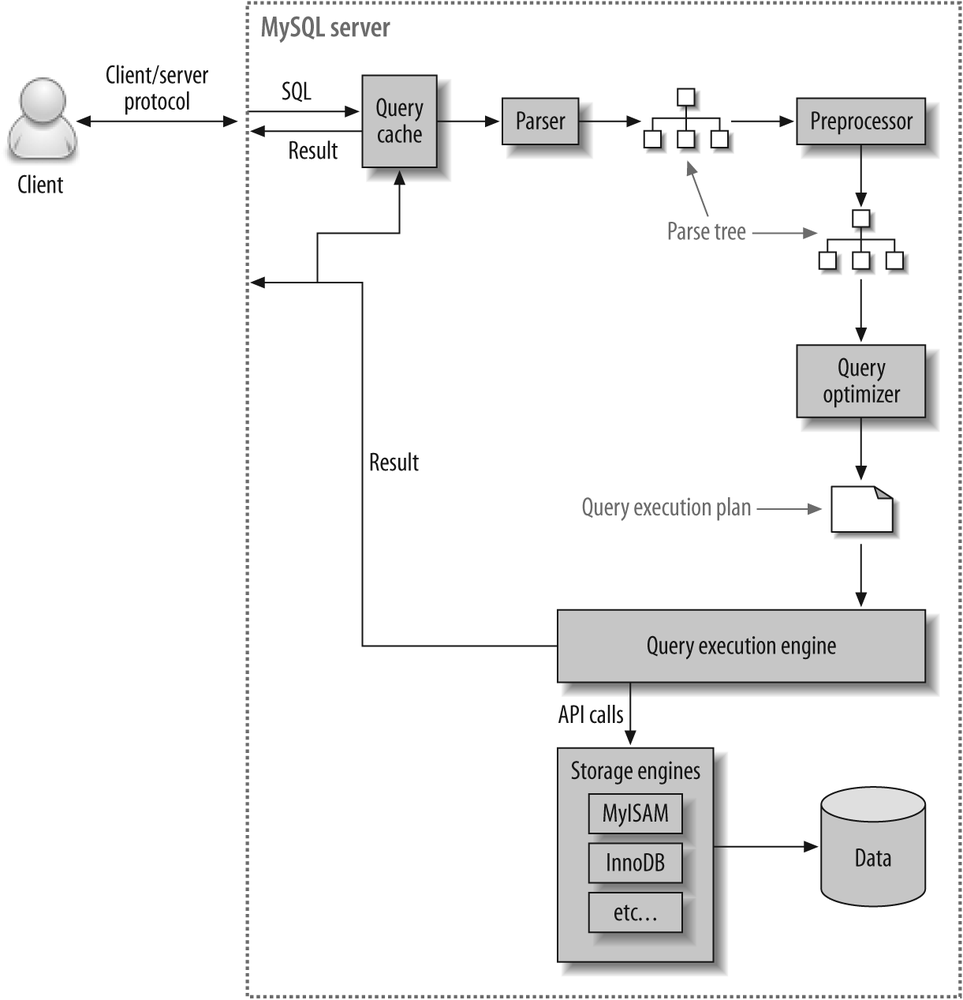
\includegraphics[scale=0.35]{files/mysql.png}
    \caption{Execution path of a query in MySQL. Taken from \parencite{QueryOptimizationBook}.}
    \label{querie_execution}
\end{figure}


\subsection{The Parser and the Preprocessor}
\label{parserAndPrepocessor}
The first step after a query cache miss, is that the parser breaks the SQL query into several parts and validates them. With theses parts, it builds a \say{parse tree} according to the syntactical scheme of relational algebra \parencite{DatabaseJournal}.

Then, the preprocessor checks the resulting tree for other semantic errors that the parser may not have been able to detect and solve. It checks that the tables and columns used in the query exist, and resolves their names and aliases to guarantee that they aren't ambiguous. Finally, the preprocessor checks the user's privileges to make sure that he can perform said query \parencite{QueryOptimizationBook}.


\subsection{The Query Optimizer}
\label{queryOptimizer}
Now that there is a valid parse tree, the query optimizer will turn it into a query execution plan \parencite{QueryOptimizationBook}. Seen as there can be several different ways of executing the same query, there are multiple execution plans and it is the optimizer's job to find the best one, according to the estimated execution performance.

First, the optimizer expands the parse tree, forms multiple alternative execution plans and then tries to predict their execution cost and choose the least expensive one. The estimation of the execution costs is based on statistics, such as:
\begin{itemize}
    \item The number of pages per table or index;
    \item The cardinality of indexes;
    \item The length of rows and keys;
    \item The key distribution.
\end{itemize}

Even though MySQL caches recently used pages in the buffer pool, the optimizer does not include the effects of any type of caching in its estimates, assuming every read will result in a disk I/O operation.

It is important to note that the chosen plan, though it might not always be optimal, will at least be near optimal. There are several reasons for this:
\begin{itemize}
    \item The statistics could be wrong. For example, the InnoDB storage engine doesn't maintain accurate statistics about the number of rows in a table;
    \item The cost metric is not exactly equivalent to the true cost of running the query, so even when the statistics are accurate, the query may be more or less expensive than the estimate;
    \item MySQL’s idea of optimal might not match the user's. Sometimes, MySQL doesn't use cost-base optimization and uses predefined rules;
    \item MySQL doesn't take concurrent running queries into account;
    \item The optimizer doesn't consider the cost of operations that are not under its control, such as executing stored functions or user-defined functions;
    \item A single query can have an infinite number of possibilities of execution plans and the optimizer can’t always estimate every possible one, so it may miss an optimal plan.
\end{itemize}

MySQL performs two types of optimization:
\begin{enumerate}
    \item \textbf{Static Optimizations:} Can be performed simply by inspecting the parse tree. For example, the optimizer can transform clauses into equivalent forms by applying algebraic rules. They can be performed once and will always be valid, even when the query is re-executed with different values. They are a kind of \say{compile-time optimization};
    
    \item \textbf{Dynamic Optimizations:} Are based on context and can depend on many factors, such as table and index statistics and which value is in a clause. They must be reevaluated each time the query is executed. They are a kind of \say{run-time optimization}. 

\end{enumerate}


\subsection{Optimizing through Indexes}
\label{optimizingIndexes}
As we have seen in Section \ref{indexingHashing}, MySQL automatically creates clustered indexes, indexes for the primary key of each table that contains all the row data. These are very important in time-sensitive queries, so the user should always define a set of primary key columns for each table \parencite{OptimizingInnoDBQueries}.

The user should also remember that the primary key columns are duplicated in all secondary indexes. As such, they should not specify too many or too long columns in the primary key, because it will reduce the performance.

The user should not create a separate secondary index for each column, because each query can only make use of one index. If the user creates indexes on columns that are rarely tested or columns with very few distinct values, they might not be helpful.

If many queries are made to the same table, it is smart to test indexes with different combinations of columns or experiment with a small number of concatenated indexes instead of a large number of single-column indexes. If an index contains all the columns needed for the query result, the query might not even read the table data.

The user should always specify if a column cannot contain NULL values using \verb|NOT NULL|. This helps the optimizer determine which index is most effective to use for a query.


\subsection{Optimizing Simple Operations}
\label{simpleOperations}


\subsubsection{The WHERE clause}
\label{whereClause}
The optimization of the \verb|WHERE| clause is done using a series of transformations and operations, such as \parencite{WHEREClauseOptimization}:
\begin{itemize}
    \item \textbf{Removal of unnecessary parentheses:}
    \begin{verbatim}
    ((a AND b) AND c OR (((a AND b) AND (c AND d))))
    
    RESULT: (a AND b AND c) OR (a AND b AND c AND d)
    \end{verbatim}
    
    \item \textbf{Replacement of constants for values:}
    \begin{verbatim}
    (a<b AND b=c) AND a=5
    
    RESULT: b>5 AND b=c AND a=5
    \end{verbatim}
    
    \item \textbf{Removal of constant conditions:}
    \begin{verbatim}
    (b>=5 AND b=5) OR (b=6 AND 5=5) OR (b=7 AND 5=6) 

     RESULT: b=5 OR b=6
    \end{verbatim}

\end{itemize}

There are many other optimizations that can be done for the \verb|WHERE| clause. However, we will not detail them in this report.


\subsubsection{The ORDER BY clause}
\label{orderByClause}
There are two strategies for optimizing the \verb|ORDER BY| clause \parencite{ORDERBYClauseOptimization}:

\vspace{0.3cm}

\noindent \textbf{Using Indexes} 

First, MySQL checks if it can use an index. This method is the best if the index contains all columns needed for the result. However, if the query contains columns which are not in the index, it may require the look up of table rows that are not indexed, making it more expensive than scanning the table and sorting the results.

\vspace{0.3cm}

\noindent \textbf{Using Filesort} 

If an index cannot be used to satisfy an \verb|ORDER BY| clause, an operation that reads table rows and sorts them is used - the \verb|filesort| operation.

The optimizer uses the \verb|sort_buffer_size| variable to allocate a memory buffer, but it increases it as needed. Because of this, this variable can be set to larger values in order to improve large sorts, without consuming excessive memory in smaller sorts. If a large amount of space that doesn't fit in memory is needed, the optimizer uses a temporary disk file.


\subsubsection{The GROUP BY clause}
\label{groupByClause}
The most basic way to satisfy a \verb|GROUP BY| clause is to perform a Full Table Scan and create a new temporary table where all rows from each group are consecutive \parencite{GROUPBYClauseOptimization}. Then this temporary table is used to find groups and apply aggregate functions, if there are any to apply.

However, in some cases, MySQL is able to perform much better and avoid the creation of temporary tables altogether by using indexes. The most important conditions for using indexes are that all \verb|GROUP BY| columns reference attributes from the same index and that the index stores its keys in order. There are two ways to execute a \verb|GROUP BY| query through index access:
\vspace{0.3cm}

\noindent \textbf{Loose Index Scan} 

The most efficient way to do a \verb|GROUP BY| is when an index is used to directly retrieve the grouping columns. Because the keys are ordered in B+-tree indexes, this enables the use of lookup groups without having to take into account all keys in the index that satisfy all \verb|WHERE| conditions. 

When there is no \verb|WHERE| clause, a Loose Index Scan reads as many keys as the number of groups, which may be a much smaller number than that of all keys. If the \verb|WHERE| clause contains range predicates, a Loose Index Scan looks up the first key of each group that satisfies the range conditions and reads the smallest possible number of keys. This is only possible if the following conditions are met:

\begin{itemize}
    \item The query is performed on a single table;

    \item The \verb|GROUP BY| only has columns that form a leftmost prefix of the index and no other columns. If a table has an index on \verb|(c1, c2, c3)|, this algorithm is only applicable if we have \verb|GROUP BY c1, c2|. It is not applicable if we have \verb|GROUP BY c2, c3| or \verb|GROUP BY c1, c2, c4|;

    \item The aggregate functions used in the select are \verb|MIN()| or \verb|MAX()|, and all of them refer to the same column. This column must be in the index and must immediately follow the columns in the \verb|GROUP BY|;

    \item All other parts of the index that are not in the \verb|GROUP BY| must be referenced in equalities with constants;

    \item Full columns values must be indexed, not just prefixes. 
\end{itemize}

\vspace{0.3cm}
\noindent \textbf{Tight Index Scan} 

When we can't use a Loose Index Scan, it may still be possible to avoid the creation of temporary tables. If there are range conditions in the \verb|WHERE| clause, the Tight Index Scan reads only the keys that satisfy these conditions. Otherwise, it performs an Full Index Scan. The grouping operation is performed after all needed keys have been found.


\subsubsection{The JOIN clause}
\label{joinClause}
When executing joins between tables, MySQL uses the Nested-Loop join algorithm or the Block Nested-Loop join algorithm \parencite{NestLoopJoinAlgorithms}. However, since version 8.0.18, MySQL began employing the Hash join algorithm for any query in which each join has an equi-join condition and uses no indexes \parencite{HashJoinOptimization}.

\begin{itemize}
    \item \textbf{Nested-Loop Join Algorithm:} This algorithm reads rows from the outer table of a loop one at a time, passing each row to an inner loop that processes the next table in the join.

    \item \textbf{Block Nested-Loop Join Algorithm:} This algorithm reads blocks of rows in the outer loop to reduce the number of times that tables in inner loops must be read.

    \item \textbf{Hash Join Algorithm:} This algorithm uses a hash function to partition the tuples of both tables and then performs the join in each of the partitions. This is usually faster than the Block Nested-Loop algorithm when there are equi-joins or natural joins.
\end{itemize}

These algorithms were studied in the lectures, so we will not go into more detail about their implementations.

In the next sections, we will talk about the optimizations and simplifications done by MySQL when processing the \verb|JOIN| clause.

\subsubsubsection{OUTER and INNER JOIN}

MySQL outer joins include the \verb|LEFT JOIN| and the \verb|RIGHT JOIN|, but internally the optimizer converts any \verb|RIGHT JOIN| into the equivalent \verb|LEFT JOIN|, by reversing its roles, like so \parencite{OuterJoinSimplification}:
\begin{verbatim}
    T1 RIGHT JOIN T2 ON P(T1, T2)

    RESULT: T2 LEFT JOIN T1 ON P(T1, T2)
\end{verbatim}

All inner join expressions of the form \verb|T1 INNER JOIN T2 ON P(T1,T2)| are replaced by the list \verb|T1,T2, P(T1,T2)| and joined with the \verb|WHERE| condition as well.

If a query with a \verb|LEFT JOIN| has a \verb|WHERE| condition that is always false for the generated NULL row, the \verb|LEFT JOIN| is changed to an inner join, like so \parencite{OuterJoinOptimization}:
\begin{verbatim}
    SELECT * FROM t1 LEFT JOIN t2 ON (column1) WHERE t2.column2=5;

    RESULT: SELECT * FROM t1, t2 WHERE t2.column2=5 
            AND t1.column1=t2.column1;
\end{verbatim}


\subsection{Optimizing Complex Operations}
\label{complexOperations}

\subsubsection{Materialization}
\label{materialization}

The optimizer uses materialization as an strategy to make the processing of subqueries more efficient. Materialization consists of storing subquery results in a temporary table and, when the results are needed again, MySQL simply reads them \parencite{Materialization}.

If possible, this method uses an in-memory temporary table. If the table is too large, it uses on-disk storage.

This optimization strategy is used by default \parencite{SwitchableOptimizations}. However, if the user wants to disable it they can simply do:

\begin{verbatim}
    SET [GLOBAL|SESSION] optimizer_switch='materialization=off';
\end{verbatim}


\subsection{Controlling the Query Optimizer}
\label{controllingQueryOptimizer}
MySQL has many ways of controlling the query optimizer. It can use system variables, which are used in switchable optimizations and also affect how query plans are chosen and evaluated. Besides that, it can use optimizer hints \parencite{ControllingOptimizer}.


\subsubsection{Number of Evaluated Plans}
\label{numberEvalutedPlans}
Regarding the number of plans that the optimizer evaluates, the user can control them by using two system variables \parencite{ControllingQueryPlanEval}:
\begin{enumerate}
    \item The \verb|optimizer_prune_level| variable tells the optimizer to skip certain plans based on estimates of the number of rows accessed for each table. This usually reduces query compilation times dramatically and is turned on by default - \verb|optimizer_prune_level=1|;
    
    \item The \verb|optimizer_search_depth| variable tells the optimizer how deeply he should look into each incomplete plan to know if it should be expanded any further. This variable should be used very carefully because it can make the compile time vary from less than a minute to several hours. If the user is unsure of what a reasonable value is, this variable should be set to 0 to tell the optimizer to determine the value automatically.
\end{enumerate}


\subsubsection{Switchable Optimizations}
\label{switchableOptimizations}
The \verb|optimizer_switch| system variable is used to gain control over optimizer behavior. This variable is set by using flags that specify the wanted optimizer behavior and it can be enabled or disabled by using \verb|on| and \verb|off|. This variable also has global and session values and can be changed at runtime \parencite{SwitchableOptimizations}.

It is important to note that, any changes to the \verb|optimizer_switch| variables affect execution of all subsequent queries and, to affect one query differently from another it is necessary to change the variables before each one.

An example of the use of these variables has been shown before with materialization, in the Section \ref{materialization}.

\vspace{0.3cm}
\noindent To switch off the use of Block Nested-Loops you could use the following instruction:
\begin{verbatim}
    SET [GLOBAL|SESSION] optimizer_switch='block_nested_loop=off';
\end{verbatim}


\subsubsection{Optimizer Hints}
\label{optimizerHints}
A way of controlling the optimizer is to specify optimizer hints inside individual statements. Hints within a statement take precedence over switching the \verb|optimizer_switch| flags \parencite{OptimizerHints}.

\vspace{0.3cm}
\noindent To force a specific join order you could use the following hint:
\begin{verbatim}
    SELECT/*+ JOIN_ORDER(t1,t2)*/ * 
    FROM t1 INNER JOIN t2 
    WHERE ...
\end{verbatim}

\vspace{0.3cm}
\noindent To force or ignore the use of an index you could use the following hints \parencite{IndexHints}:
\begin{verbatim}
    SELECT * 
    FROM t1 USE INDEX(col1Index,col2Index)
    WHERE ...
    
    SELECT * 
    FROM t1 IGNORE INDEX(col3Index)
    WHERE ...
\end{verbatim}

\vspace{0.3cm}
\noindent To force the use of a specific join algorithm you could use the following hint \parencite{OptimizerHints}:
\begin{verbatim}
    SELECT /*+ NO_BNL() HASH_JOIN(t1,t2)*/*
    FROM t1 INNER JOIN t2 INNER JOIN t3
\end{verbatim}

\vspace{0.3cm}
\noindent To set system variables for the duration of the statement you could use the following hint \parencite{OptimizerHints}:
\begin{verbatim}
    INSERT /*+ SET_VAR(foreign_key_checks=OFF) */ 
    INTO t2 VALUES(2);
\end{verbatim}


\vspace{0.3cm}

Concluding Section \ref{controllingQueryOptimizer}, it is best not to try to outsmart the optimizer. By doing this, you may end up defeating its purpose.

However, it is important to note that sometimes you may know something about the data that the optimizer doesn't. This frequently happens with database administrators or users that know a database inside out. If you know for sure that the optimizer isn't giving you good results, and you know why, you can help it by using the tools described in this section.



\subsection{Estimating Table and Index Statistics}
\label{estimativas}
The estimation of query performance is made by counting the number of disk seeks. When using B+-tree indexes, you need this many seeks to find a row \parencite{EstimatingPerformance}:
\begin{equation}
\frac{log(row\_count)}{log(\frac{index\_block\_length}{3} * \frac{2}{ (index\_length + data\_pointer\_length)}}
+ 1
\end{equation}


\vspace{0.3cm}

Optimizer statistics are persisted to disk by default. If you turn this behaviour off by using \verb|innodb_stats_persistent=OFF| or create tables with \verb|STATS_PERSISTENT=0|, statistics are not persisted to disk \parencite{InnoDBStatisctsEstimation}. Instead, they are stored in memory, and are lost when the server shuts down. Statistics are also updated periodically by certain operations and under certain conditions.

To update non-persistent optimizer statistics you could:
\begin{itemize}
    \item Run \verb|ANALYZE TABLE|;
    
    \item Run \verb|SHOW TABLE|;
    
    \item Run \verb|SHOW INDEX|;
    
    \item Query \verb|INFORMATION_SCHEMA.TABLES| or \verb|INFORMATION_SCHEMA.STATISTICS| with the \verb|innodb_stats_on_metadata| option enabled.

\end{itemize}



\subsection{The Execution Plan}
\label{executionPlan}
After the parsing and optimizing stages, a query execution plan is outputted. This plan is used by the query execution engine to process the query. Contrary to many other databases, in MySQL this plan is not byte-code but a tree of instructions \parencite{QueryOptimizationBook}.

After executing the plan, the results are sent back to the client. It is important to note that the server generates and sends results incrementally. If the query is cacheable, MySQL will also place the results into the query cache. 

\vspace{0.3cm}

To display detailed information from the optimizer about a statement execution plan, we use \verb|EXPLAIN| with an explainable statement: \verb|SELECT|, \verb|DELETE|, \verb|INSERT|, \verb|REPLACE| or \verb|UPDATE|. MySQL explains how it would process the statement, including information about how tables are joined and in which order \parencite{ExplainStatement}. 

\vspace{0.3cm}
\noindent The syntax to use the EXPLAIN statement is the following \parencite{ExplainStatementOutput}:
\begin{verbatim}
    EXPLAIN
    SELECT t1.a, t1.a IN (SELECT t2.a FROM t2) FROM t1;
\end{verbatim}


\subsection{Comparison with Oracle 18c}
\label{optimizingComp} 
Generally speaking, the Oracle optimizer is very similar to the MySQL optimizer, in the sense that it performs query transformations and optimizations in order to obtain better performance. Just like in MySQL, Oracle stores estimations of table and index statistics to use when evaluating the cost of an execution plan.

However, when you delve into the details of Oracle's optimization, you can clearly see that it is more complete. Besides performing materialization, as MySQL does, it also allows pipelining. Furthermore, besides implementing the Full Table and Index Scans, Oracle implements several others, such as \parencite{OptimizerAccessPaths}:
\begin{itemize}
    \item Table access by row id;
    \item Sample Table Scan;
    \item Index Fast Full Scan;
    \item Index Skip Scans;
    \item Index Join Scans;
    \item In-Memory Dynamic Scans;
    \item Etc.
\end{itemize}

As for the join algorithms available, Oracle provides one more than MySQL, the Sort Merge join \parencite{JoinMethods}.

Both MySQL and Oracle allow the user to specify which indexes and algorithms to use through hinting within statements. 

Lastly, just like MySQL does, Oracle has an instruction that allows the user to see the details of the execution plan.
 




\newpage
\section{Transaction Management and Concurrency Control}
\label{transactionAndConcurrency}

\subsection{Transactions}
\label{transactions} 
A transaction is a unit of program execution that accesses and possibly
updates various data items in a database \parencite{AulaTransactions}. To preserve the integrity of data, the InnoDB storage engine adheres closely to the ACID model. Its properties guarantee that data is not corrupted and results are not distorted by exceptional conditions, such as software crashes and hardware malfunctions \parencite{innodbACID}.

\vspace{0.3cm}

\noindent Below, we present an example of how to start a transaction in MySQL, then update a table and commit the changes \parencite{transactionIsolationLevels}:

\begin{verbatim}
    START TRANSACTION;
    UPDATE t SET b = 5 WHERE b = 3;
    COMMIT;
\end{verbatim}

\noindent If, instead of committing the changes, the user wanted to cancel all modifications made by the current transaction, he could just use the \verb|ROLLBACK;| statement.

\vspace{0.3cm}

In MySQL, transactions cannot be nested. This happens due to the implicit commit performed for any current transaction when you use the \verb|START TRANSACTION| statement \parencite{implicitCommit}.

However, it is possible for a user to \say{mimic} this functionality by using savepoints \parencite{nestedMySQL}.

\vspace{0.3cm}

As we said before, the transactions implemented by InnoDB have ACID properties. Long Duration Transactions are transactions that take a lot of time, so it is unlikely that isolation can be guaranteed. Without isolation, the atomicity may be compromised and, as such, this kind of transaction isn't implemented by InnoDB.


\subsection{The ACID Model}
The following sections discuss how the InnoDB storage engine deals with the categories of the ACID model.

\subsubsection{Atomicity}
\label{atomicity} 
In the ACID model, the A stands for Atomicity. Atomicity ensures that, within a transaction, either all operations are properly reflected in the database or none are \parencite{AulaTransactions}. MySQL with InnoDB engine guarantees this property by using the following features \parencite{innodbACID}:

\begin{itemize}
    \item \textbf{Autocommit Setting:} By default, MySQL has the autocommit setting turned on. This setting treats each statement as atomic and commits the work after said statement has finished. If an error occurs during the statement execution a rollback statement is issued;
    
    \item \textbf{Commit Statement:} MySQL with InnoDB engine implements the \verb|COMMIT| statement, which makes the current transaction's changes permanent. If you have autocommit enabled, it automatically commits after each statement. Because of this, the user should only use the \verb|COMMIT| statement when a \verb|START TRANSACTION| was issued or when autocommit is turned off;
    
    \item \textbf{Rollback Statement:} MySQL with InnoDB engine implements the \verb|ROLLBACK| statement, which cancels the current transaction's changes. As explained above, this statement is used when a \verb|START TRANSACTION| is issued or when autocommit is turned off;

    \item \textbf{Information Schema table:} With the \verb|INFORMATION_SCHEMA| table, \verb|INNODB_TRX|, we can check information about every transaction that is executing inside InnoDB. When using this table, we can see the transaction state, when the transaction started and the particular SQL statement the transaction is executing \parencite{InformationSchemaTransactionLockingInfo}.
    
\end{itemize}


\subsubsection{Consistency}
\label{consistency} 
In the ACID model, the C stands for Consistency. Consistency ensures that when the execution of a transaction ends, it preserves the state of the database \parencite{AulaTransactions}. Guaranteeing the consistency property essentially involves internal InnoDB processing to protect data from crashes. MySQL with InnoDB engine guarantees this property by using the following features \parencite{innodbACID}: 

\begin{itemize}
    \item \textbf{Doublewrite Technique:} This technique allows InnoBD to recover a page in case of a system crash in the middle of a page write, because it keeps a copy of said page in the doublewrite buffer. In a nutshell, InnoDB first writes and flushes pages to the doublewrite buffer. Finally, after it has completed the write and flush, InnoDB writes the pages to their correct positions in the data file \parencite{doublewriteBufferGloss};

     \item \textbf{Crash Recovery:} After a crash, when MySQL is re-started, it starts cleanup activities. These activities consists of scanning tables for incomplete transactions and then, using the redo log, starting them again. It checks for changes that were committed before the crash, but weren't written into the data files and uses the doublewrite buffer to reconstruct them. However, if the database is shut down normally, this type of activity is performed during shutdown by the purge operation \parencite{crashRecoveryGloss}.
     
\end{itemize}

\vspace{0.3cm}

In an SQL statement that inserts, deletes, or updates many rows, foreign key constraints are checked row-by-row. InnoDB sets shared row-level locks on child or parent records that it must examine and checks the constraints immediately. The check cannot be deferred to a later moment, for example to the transaction commit \parencite{fkDeferConstraint}.

\subsubsection{Isolation}
\label{isolation}
In the ACID model, the I stands for Isolation. Isolation ensures that, even though multiple transactions may execute concurrently, each one must be unaware of other concurrently executing transactions and mustn't see their intermediate results \parencite{AulaTransactions}.

Transaction isolation is at the foundation of database processing. Isolation levels allow the user to balance performance, reliability, consistency and reproducibility of results, when multiple transactions run concurrently \parencite{transactionIsolationLevels}.

InnoDB uses a combination of multi-versioning properties with traditional two-phase locking \parencite{innodbTransactionModel}. Multi-version concurrency control allows InnoDB transactions with certain isolation levels to query rows that are being updated by other transactions and see their values before those updates occurred \parencite{MVCC}.


\subsubsubsection{Isolation Levels}
\label{isolationLevels} 
InnoDB offers all four standard SQL transaction isolation levels \parencite{transactionIsolationLevels}:
\begin{enumerate}
    \item \verb|READ UNCOMMITTED|: Uncommitted records can be read. \verb|SELECT| statements are performed without using locks. When using this isolation level, reads are not consistent and are also called a dirty reads;
    
    \item \verb|READ COMMITTED|: Only committed records can be read. However, each consistent read, even within the same transaction, sets and reads its own fresh snapshot. This means that successive reads of a record may return different committed values;
    
    \item \verb|REPEATABLE READ|: This is the default isolation level for InnoDB. Only committed records can be read. However, consistent reads within the same transaction read the snapshot established by the first read. This means that the record values read within each transaction will always be consistent with each other;
    
    \item \verb|SERIALIZABLE|: Completely isolates the effects of one transaction from all others. Tries to ensure that transactions run in such a way that they appear to be executed one at a time, rather than concurrently.
\end{enumerate}

\vspace{0.3cm}

InnoDB supports each of the transaction isolation levels described using different locking strategies. 

If the user wants to perform operations that need a high degree of consistency, the \verb|REPEATABLE READ| isolation level can be used. On the other hand, if the user wants to perform operations with a lower the degree of consistency, he can do so by using \verb|READ COMMITTED| or \verb|READ UNCOMMITTED|. For stricter rules than the repeatable read, the user may choose the \verb|SERIALIZABLE| level.

\vspace{0.3cm}

\noindent The user can change the isolation level for a single session or for all subsequent connections like so \parencite{setTransaction}:

\begin{verbatim}
SET [GLOBAL | SESSION] TRANSACTION ISOLATION LEVEL SERIALIZABLE;
\end{verbatim}


\subsubsubsection{Savepoints}
\label{savepoints} 
With the InnoDB engine, the user can make use of savepoints \parencite{savepoints}. The following code creates a transaction savepoint with a name of identifier: 

\begin{verbatim}
    SAVEPOINT transaction_id1;
\end{verbatim}

It is important to note that, if the current transaction has a savepoint with the same name, the old savepoint is deleted and a new one is set.

\vspace{0.3cm}

To undo the modifications that the current transaction made to rows after the savepoint was set, the user can use the following code:
\begin{verbatim}
    ROLLBACK TO SAVEPOINT transaction_id1;
\end{verbatim}

Note that savepoints that were created at a later time than the named savepoint are deleted.

\vspace{0.3cm}

To remove a named savepoint from the set of savepoints of the current transaction without performing a commit or a rollback, the user can use the following code:
\begin{verbatim}
    RELEASE SAVEPOINT transaction_id1;
\end{verbatim}

If the user issues a \verb|COMMIT| or a \verb|ROLLBACK| statement, all savepoints of the current transaction are deleted.


\subsubsection{Durability}
\label{durability} 
In the ACID model, the D stands for Durability. Durability ensures that after a transaction completes successfully, the changes it has made to the database persist, even if there are system failures \parencite{AulaTransactions}.

Guaranteeing durability with MySQL involves software features interacting with particular hardware configurations. There are many possibilities that depend on the capabilities of the CPU, network and storage devices. We will not go into detail about these specifications because it is very hard to provide guidelines for them \parencite{innodbACID}.

However, as we mentioned in Section \ref{consistency}, InnoDB uses the doublewrite buffer as a storage area to write pages flushed from the buffer pool, before writing them to their corresponding positions in the data files \parencite{DoubleWriteBuffer}. This guarantees that, if there is a system crash, InnoDB can find good copies of the pages in the doublewrite buffer during crash recovery.

Even though data is written twice, this doesn't require twice as much I/O overhead or operations, because the data is written to the doublewrite buffer in a large sequential chunk, with a single \verb|fsync()| call to the operating system.



\subsection{Concurrency Control}
\label{concurrencyControl}

\subsubsection{Lock Granularity}
\label{lockGranularity} 
InnoDB implements standard row-level locking where there are two types of locks \parencite{innoDBLocking}:

\begin{enumerate}
    \item \textbf{Shared (S) Locks:} Allow the transaction that holds the lock to read a row;
    
    \item \textbf{Exclusive (X) Locks:} Allow the transaction that holds the lock to update or delete a row.
\end{enumerate}


If transaction \verb|T1| holds an S lock on \verb|row r| and another transaction \verb|T2| requests a lock on the same row, then:

\begin{itemize}
    \item If \verb|T2| requested an S lock, it can be granted immediately. This means that both \verb|T1| and \verb|T2| now hold an S lock on \verb|row r|;
    
    \item If \verb|T2| requested an X lock, it cannot be granted immediately.

\end{itemize}

\vspace{0.3cm}

If transaction \verb|T1| holds an X lock on \verb|row r| and another transaction \verb|T2| requests either type of lock on the same row, then it cannot be granted immediately, and \verb|T2| has to wait for the lock to be released.

\vspace{0.3cm}

Because InnoDB supports multiple granularity locking, it allows for the coexistence of row locks and table locks. 

So, InnoDB implements intention locks, table-level locks that specify which type of lock a transaction requires later for a row in a table. There are two types of intention locks:

\begin{enumerate}
    \item \textbf{Intention Shared (IS) Locks:} Specify that a transaction intends to set an S lock on individual rows in a table;
    
    \item \textbf{Intention Exclusive (IX) Locks:} Specify that a transaction intends to set an X lock on individual rows in a table.
    
\end{enumerate}

\vspace{0.3cm}

With intention locking, before a transaction can acquire an S lock on a table row, it must first acquire an IS lock or stronger on the table.

Additionally, before a transaction can acquire an X lock on a table row, it must first acquire an IX lock on the table.

\newpage
To obtain an IS lock, use the following code:
\begin{verbatim}
    SELECT * FROM table1
    WHERE id = 1
    FOR SHARE;
\end{verbatim}

To obtain an IX lock, use the following code:
\begin{verbatim}
    SELECT * FROM table1
    WHERE id = 1
    FOR UPDATE;
\end{verbatim}

Table \ref{locksTable} represents the compatibility of Table-level lock types:
\begin{table}[h!]
\caption{Table-Level Lock Type Compatibility}
\centering
\begin{tabular}{ |p{2cm}||p{2cm}|p{2cm}|p{2cm}|p{2cm}|   }
 \hline
  & X & IX & S & IS\\
 \hline
 X & Conflict & Conflict & Conflict & Conflict\\
 IX & Conflict & Compatible & Conflict & Compatible\\
 S & Conflict & Conflict & Compatible & Compatible\\
 IS & Conflict & Conflict & Compatible & Compatible\\
 \hline
\end{tabular}
\label{locksTable}
\end{table}

\vspace{0.3cm}

A lock is only granted to a transaction if it is compatible with all other existing locks. Otherwise, a transaction waits until the conflicting existing lock is released. However, if there is a conflict with an existing lock that cannot be granted because it would cause a deadlock, an error occurs. Details on how InnoDB deals with deadlocks will be given in Section \ref{deadLocks}.

The goal of intention locks is to show that someone is locking a row, or going to lock a row in a table. As such, intention locks do not block anything except full table requests:

\begin{verbatim}
    LOCK TABLE table1 WRITE;
\end{verbatim}


\subsubsection{Row-Level Locks}
\label{rowLevelLocks} 

\begin{itemize}
    \item \textbf{Record Lock:} A lock on an index record. This type of lock prevents any other transaction from inserting, updating or deleting rows from an index record. They lock the index record even if there is no index on such table, due to the existence of the clustered index;
    
    \vspace{0.3cm}
    The following code prevents any other transaction from inserting, updating, or deleting rows where the value of \verb|t.c1| is 10:
\begin{verbatim}
SELECT c1 FROM t WHERE c1 = 10 FOR UPDATE;
\end{verbatim}
    
    
    \item \textbf{Gap Lock:} Locks all index records within a range, or the gap before the first or after the last index record. In InnoDB, the purpose of a Gap Lock is to prevent other transactions from inserting to the gap so, multiple Gap Locks can co-exist;
    
    \vspace{0.3cm}
    The following code prevents any other transactions from inserting values between 10 and 20 into column \verb|t.c1|: 
\begin{verbatim}
SELECT c1 FROM t WHERE c1 BETWEEN 10 and 20 FOR UPDATE;
\end{verbatim}

    \item \textbf{Next-Key Lock:} A lock that is a combination of a Record lock on an index record and a Gap lock on the gap before that index record. A Next-Key lock on an index record also affects the gap between that record and the one before it. For example, suppose that an index contains the values 10, 11, 13, and 20. If a Next-Key lock is created for record 20 in the index, another session cannot insert a new index record in the gap between 13 and 20;
    
    \item \textbf{Insert Intention Locks:} A type of Gap lock that is set for \verb|INSERT| operations. This lock allows multiple transactions to insert into the same index gap without waiting for each other, if they are not inserting at the exact same position within the gap.

\end{itemize}

\subsubsection{Deadlocks}
\label{deadLocks} 
A deadlock is a situation in which different transactions are unable to proceed because each of them holds a lock that the other needs. This happens because both transactions are waiting for a resource to become available, while holding a resource that the other transaction needs. This situation can occur, for example, when transactions lock rows in multiple tables in the opposite order\parencite{deadlocksInInnoDB}.

Below, we illustrate how a deadlock can occur in MySQL. The following example involves two clients, A and B \parencite{deadlockExample}:

\begin{verbatim}
    /* Client A inserts one row into a table, then
    starts a transaction and obtains
    an S lock on the row */

    INSERT INTO t (id) VALUES(1);
    START TRANSACTION;
    SELECT * FROM t WHERE id = 1 FOR SHARE;
\end{verbatim}

 
\begin{verbatim}
    /* Client B starts a transaction and tries to 
    delete the same row from the table */
    
    START TRANSACTION;
    DELETE FROM t WHERE id = 1;    
\end{verbatim}

The delete operation requires an X lock that cannot be granted because it is incompatible with the S lock that client A has. So, client B is blocked while waiting for client A to release his S lock.

\begin{verbatim}
    /* Client A also attempts to delete the
    same row from the table */
    
    DELETE FROM t WHERE id = 1;
\end{verbatim}

Deadlock occurs because client A needs an X lock to delete the row. That lock cannot be granted because client B already requested an X lock and is waiting for client A to release its S lock. The S lock held by A cannot be upgraded to an X lock because of the prior request by B for an X lock. So, InnoDB generates an error for one of the clients, releases its locks and grants the other clients lock.

\subsubsubsection{Deadlock Detection and Rollback}
\label{deadlockDetection}
In MySQL, deadlock detection is enabled by default. When InnoDB detects a deadlock, it chooses a transaction to roll back, the victim. When choosing the victim, InnoDB tries to pick small transactions to roll back, with the size of a transaction being determined by the number of rows inserted, updated, or deleted \parencite{deadlockdetectionAndRollback}.

When deadlock detection is disabled by using the \verb|innodb_deadlock_detect| configuration option, InnoDB relies on the \verb|innodb_lock_wait_timeout| setting to roll back transactions in case of a deadlock.

\subsubsubsection{Minimizing Deadlocks}
To diminish the possibility of deadlocks, MySQL recommends: 
\begin{itemize}
    \item Using transactions instead of locking tables;
  
    \item Keeping transactions as small and short as possible in order to avoid collisions;
    
    \item When modifying multiple tables within a transaction, doing those operations in a consistent order each time;
    
    \item Creating indexes on columns used by the \verb|SELECT ... FOR UPDATE|  and the \verb|UPDATE ... WHERE| statements;
    
    \item Trying to re-issue a transaction if it fails due to deadlock.
\end{itemize}


\subsection{Comparison with Oracle 18c}
\label{transactionComp}
Oracle and MySQL are very alike when it comes to transactions, as both follow the ACID model. Regarding isolation levels, both implement the standard ones but have different defaults: Oracle uses the \verb|READ COMMITTED| and MySQL uses the \verb|REPEATABLE READ|. They both support the use of savepoints with similar syntax. 

When it comes to locking, they are both very similar, with the exception that Oracle allows the deferral of constraint checking, and MySQL does not \parencite{OracleConstraintDefered}.

As for deadlocks, they use the similar tactics for handling them, by choosing a victim. However, they differ on the method of choosing such victim: Oracle's victim is the transaction that detected the deadlock \parencite{OracleLocksAndDead}; MySQL's victim is the transaction with the least amount of rows inserted, updated or deleted.





\newpage
\section{Other characteristics of MySQL}
\label{otherCharacteristics}
MySQL has a lot of functionalities that do not align directly with the subjects lectured in the Database Systems course. Of those functionalities, we will present some of the ones that we found to be more interesting.

\subsection{Web Support}
\label{webSupport}
MySQL provides Web support through XML and XPath.


\subsubsection{XML Support}
\label{xmlSupport}
\subsubsubsection{Exporting XML}
\label{exportXml}
MySQL provides a way to obtain XML-formatted output by starting the \verb|mysql| or \verb|mysqldump| clients with the \verb|--xml| option \parencite{XMLFunctions}. We get the same output using either client.

\vspace{0.3cm}

\noindent Using \verb|mysql|, the command will be as follows \parencite{xmlmysqlOption}:
\begin{verbatim}
    mysql --xml -uroot -e "SHOW VARIABLES LIKE 'version%'"
\end{verbatim}

\vspace{0.3cm}

\noindent To write the output to an XML file, do as follows:
\begin{verbatim}
    mysql --xml -e 'SELECT * FROM mydb.table1' > fileName.xml
\end{verbatim}

\noindent Using \verb|mysqldump|, the command will be as follows \parencite{xmlmysqldumpOption}:
\begin{verbatim}
    mysqldump --xml -u root world City
\end{verbatim}

\subsubsubsection{Importing XML}
\label{importXml}
MySQL also allows us to import data from an XML file into a table using the \verb|LOAD XML| statement \parencite{loadXMLStatement}. This is complimentary to running the \verb|mysql| client in XML output mode. 

The following example shows how you could import data from an XML file into \verb|table1|:
\begin{verbatim}
    LOAD XML LOCAL INFILE "/dirPath/fileName.xml"
    INTO TABLE table1
\end{verbatim}


\subsubsection{XPath Support}
\label{xpathSupport}
MySQL manipulates XML data using XPath, a language for navigating and querying XML documents. For this, if offers two functions:
\begin{enumerate}
    \item \verb|ExtractValue(xml_far, xpath_expr)|;
    
    \item \verb|UpdateXML(xml_target, xpath_expr, new_xml)|.
\end{enumerate}

The \verb|ExtractValue| function receives an XML markup fragment and an XPath expression and returns the text of the first text node which is a child of the element or elements matched by the XPath expression. In case of multiple matches, they are returned as a single space-delimited string. If there are no matches, an empty string is returned.

\vspace{0.3cm}

The \verb|UpdateXML| function receives two XML markup fragments and an XPath expression. It replaces a portion of an XML fragment with the new XML fragment and returns the changed XML. The portion replaced is the one that matches the XPath expression. If no expression matching the given one is found, or if multiple matches are found, the function returns the original XML \parencite{XMLFunctions}.
 


\subsection{Stored Routines}
\label{procedures}
MySQL supports two types of stored routines: procedures and functions. A stored routine is a set of SQL statements that can be stored in the server. Then, the clients don't need to reissue the individual statements but can make a reference to the stored routine \parencite{storedRoutines}.

These stored routines can be very useful:
\begin{itemize}
    \item When multiple client applications use different languages or platforms, but need to perform the same operations;
    
    \item If security is very important, applications and users could have no access to the database tables themselves and only be able to execute specific stored routines.
    
\end{itemize}

\noindent In the following sections, we will demonstrate how to manage procedures.

\subsubsection{Create Procedure}
\label{createProcedure}
The following code shows how to create a procedure that counts the number of cities in a country \parencite{createProcedure}:

\begin{verbatim}
CREATE PROCEDURE citycount (IN country CHAR(3), OUT cities INT)
       BEGIN
         SELECT COUNT(*) INTO cities FROM world.city
         WHERE CountryCode = country;
       END;
\end{verbatim}


\subsubsection{Alter Procedure}
\label{alterProcedure}
The following code shows how to alter the previously defined procedure \parencite{alterProcedure}:

\begin{verbatim}
ALTER PROCEDURE citycount [characteristic ...]

characteristic: {
    COMMENT 'string'
  | LANGUAGE SQL
  | {CONTAINS SQL | NO SQL | READS SQL DATA | MODIFIES SQL DATA}
  | SQL SECURITY {DEFINER | INVOKER}
}
\end{verbatim}

\noindent The \verb|ALTER PROCEDURE| statement can be used to change the characteristics of a stored procedure. However, it is not possible to change the parameters or body by using this statement. In order to do that, the user must \verb|DROP| the procedure and re-create it.


\subsubsection{Drop Procedure}
\label{alterProcedure}
The following code shows how to drop the previously defined procedure \parencite{dropProcedure}:

\begin{verbatim}
DROP PROCEDURE [IF EXISTS] citycount;

\end{verbatim}



\subsection{Triggers}
\label{triggers}
A trigger is a named database object that is associated with a table. This object is activated when a particular event for that table occurs. Triggers are used to perform checks of values to be inserted into a table or to perform calculations on values involved in an update \parencite{TriggersDef}.

\vspace{0.3cm}

\noindent In the following sections, we will demonstrate how to manage triggers.

\subsubsection{Create Trigger}
\label{createTrigger}
The following code shows how to create a trigger that accumulates the values inserted into one of the columns of the table \parencite{TriggerSyntax}:
\begin{verbatim}
CREATE TRIGGER ins_sum BEFORE INSERT ON account
    FOR EACH ROW SET @sum = @sum + NEW.amount;
\end{verbatim}


\subsubsection{Drop Trigger}
\label{dropTrigger}
The following code shows how to drop the previously defined trigger:
\begin{verbatim}
DROP TRIGGER schema.ins_num;
\end{verbatim}

\noindent With the \verb|DROP TRIGGER| statement, the user must specify the schema name if the trigger is not in the default schema. Trigger names exist in the schema namespace. This means that all triggers must have unique names within a given schema.

It is important to note that when you drop a table, all the existing triggers related to that table are also dropped \parencite{TriggerSyntax}.


\subsection{JDBC DriverManager Interface}
\label{jdbc}
With MySQL, it is possible to use Java to send instructions to a database by using Java Database Connectivity (JDBC). To establish a connection, the user can import the \verb|DriverManager| class \parencite{JDBCConnector}. The following code is an example of how to create a connection and use it to query a database \parencite{executeSQL}:

\begin{verbatim}
import java.sql.Connection;
import java.sql.DriverManager;
import java.sql.SQLException;
import java.sql.Statement;
import java.sql.ResultSet;

Connection conn = null;
Statement stmt = null;
ResultSet rs = null;

try {
     conn =
       DriverManager.getConnection(
       "jdbc:mysql://localhost/test?"
        + "user=minty&password=greatsqldb");
        
    stmt = conn.createStatement();
    rs = stmt.executeQuery("SELECT foo FROM bar");
}
catch (SQLException ex){
    // Handle any errors
    System.out.println("SQLException: " + ex.getMessage());
    System.out.println("SQLState: " + ex.getSQLState());
    System.out.println("VendorError: " + ex.getErrorCode());
}
finally {
    // Release resources in this block
}
\end{verbatim}

\subsection{MySQL Workbench}
\label{workbench}
MySQL Workbench is a graphical tool for working with MySQL servers and databases. It supports MySQL version 5.5 and above, and has five main areas of functionality \parencite{workbench}:
\begin{enumerate}
    \item \textbf{SQL Development:} Allows the creation and management of connections to database servers. It provides the capability to execute SQL queries on the database connections using the Visual SQL Editor, discussed in Section \ref{visualSQLEditor};
    
    \item \textbf{Data Modeling:} Allows the creation of models of database schemas graphically and the edition of all aspects of the database;
    
    \item \textbf{Server Administration:} Allows the creation and administration of server instances;

    \item \textbf{Data Migration:} Allows migrations from Microsoft SQL Server, Sybase ASE, SQLite, SQL Anywhere, PostreSQL and other RDBMS tables, objects and data to MySQL;
    
    \item \textbf{MySQL Enterprise Support:} Provides support for Enterprise products.

\end{enumerate}


\subsubsection{Visual SQL Editor}
\label{visualSQLEditor}
The Visual SQL Editor is a set of specialized editors (query, schema, table, etc) and panels that, together, enable you to \parencite{visualSQLEditor}: 

\begin{itemize}
    \item Build, edit and run queries;
    \item Create and edit data;
    \item View and export results;
    \item Perform basic RDBMS administrative tasks.
\end{itemize}

In Figure \ref{visualEditorImage}, you can see the appearance of the Visual SQL Editor tool.

\begin{figure}[htbp]
\centering
    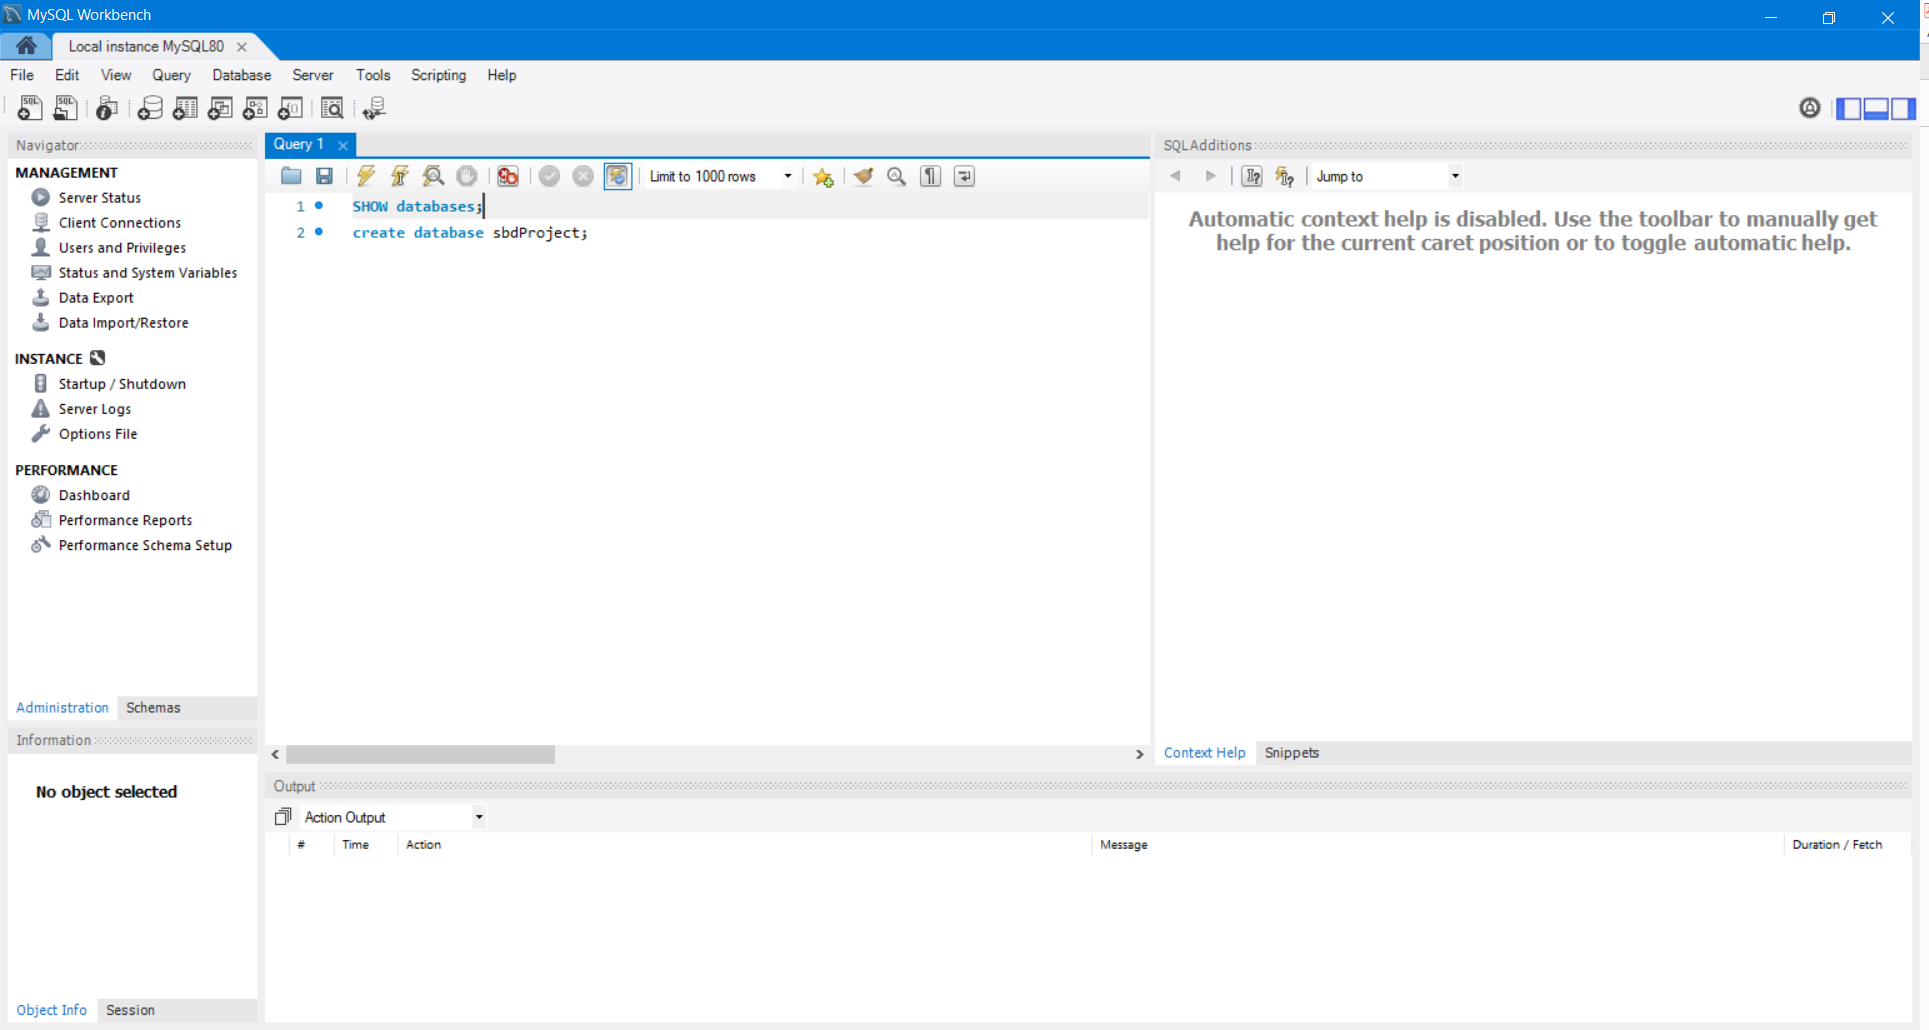
\includegraphics[scale=0.2]{files/workbench.png}
    \caption{Screenshot of Visual SQL Editor.}
    \label{visualEditorImage}
\end{figure}




\newpage
\section{Conclusion}
\label{conclusion}
Because we are Computer Science students, getting to know a new Database Management System was really important and useful to us.

Usually, the biggest issue when starting a new project is to define which technologies to use, namely the database system. So, we found the experience of researching the \say{ins and outs} of MySQL with the InnoDB storage engine very enriching and helpful in understanding two of the most popular DBMS, MySQL and Oracle.

With the knowledge we gathered in this extensive study, we will be able to use MySQL databases with more ease in future projects and applications. We believe that, the next time we have to choose DBMS for a new project, we will be more aware of the relevant characteristics to bear in mind.

Besides getting to know a new DBMS, we found that this project was also very effective in making us understand Oracle. It helped us with solidifying the subjects lectured in class and prepared us for the exam in a way that \say{regular} studying couldn't.

Overall, we found the making of this project to be a very positive experience and we believe that it was very adequate for the purpose of this course.


\newpage
\printbibliography[
heading=bibintoc,
title={References}
]

\end{document}